% git add .
% git commit -m "update"
% git push origin main            =============> push to Github
% git push overleaf main:master   =============> push to Overleaf

\documentclass[wcp]{jmlr}

\usepackage{amsmath, amssymb, booktabs, graphicx, float}
\usepackage{geometry}
\geometry{margin=1in}

\title{Portfolio Optimization, Efficient Frontier, and Asset Allocation}

\author{
\Name{Uros Markovic} \Email{uros.markovic.quant@gmail.com} \\
\addr Johns Hopkins University
}

\begin{document}

\maketitle

\begin{abstract}
This report presents a comprehensive portfolio optimization framework using historical asset returns. We construct and analyze multiple portfolio strategies, including minimum-variance, maximum-return, tangency (maximum Sharpe ratio), risk-parity, and dollar-neutral portfolios.

We extend the classical mean-variance framework by incorporating investor preferences through indifference curves, deriving optimal portfolios via utility maximization. Additionally, we establish connections to the Capital Asset Pricing Model (CAPM) and interpret the efficient frontier through Sharpe ratio iso-lines.
\end{abstract}

\section{Introduction}

Modern Portfolio Theory (MPT), introduced by Markowitz, provides a framework for balancing risk and return. This report applies the framework to a multi-asset portfolio consisting of equities (Nike, Amazon, Google, Tesla, Microsoft), using historical log-returns.

We extend the classical framework by incorporating:
\begin{itemize}
\item Utility maximization via risk aversion
\item Tangency portfolio derivation
\item Sharpe ratio geometry
\item CAPM interpretation
\end{itemize}

\section{Data and Preprocessing}

Daily adjusted closing prices are obtained from Yahoo Finance over the period 2020--2023.

\begin{figure}[H]
\centering
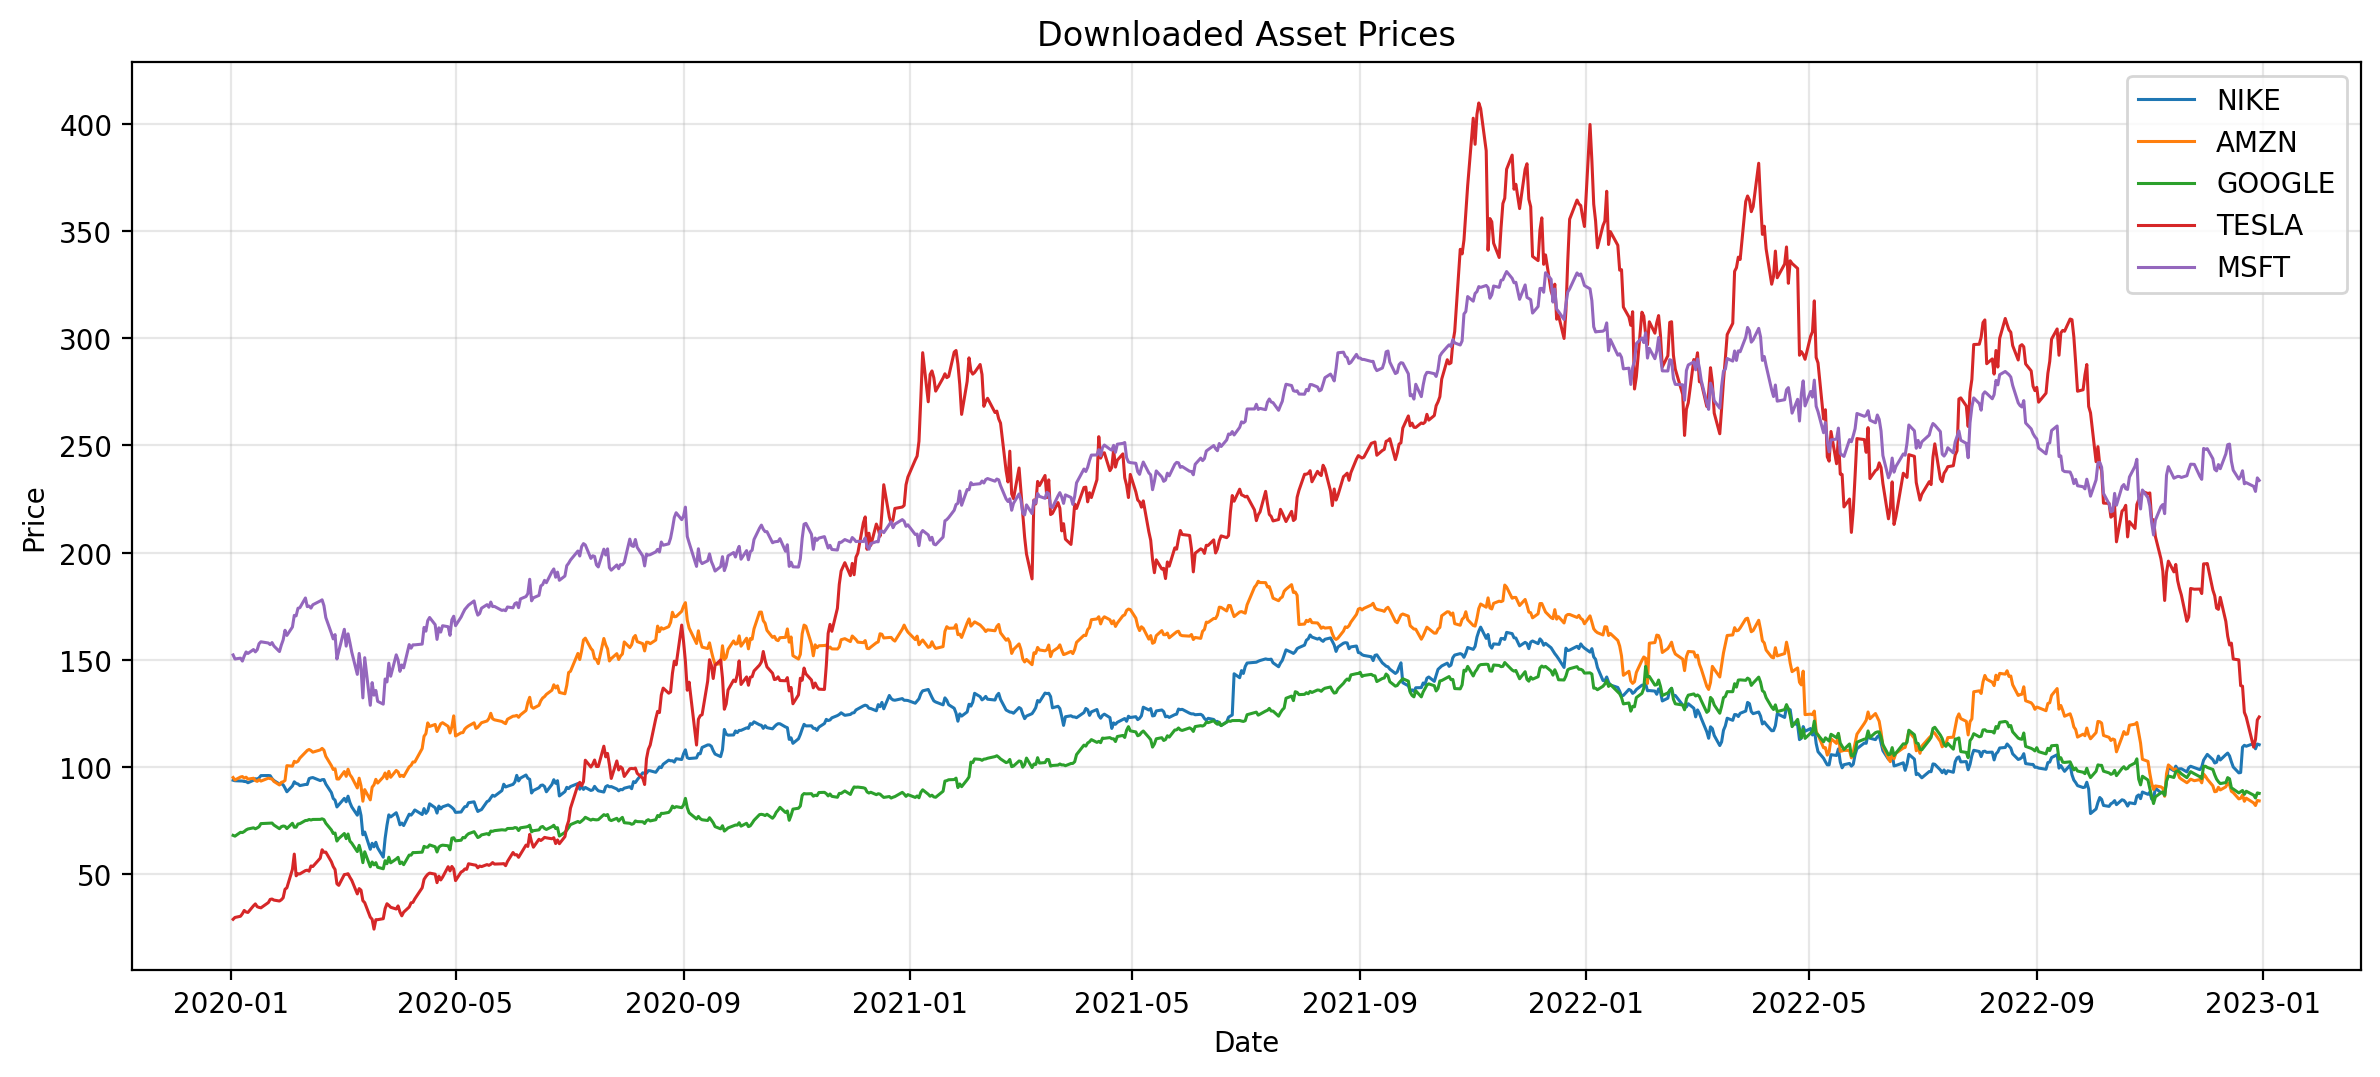
\includegraphics[width=0.9\textwidth]{outputs/figures/01_prices.png}
\caption{Asset price evolution}
\label{fig:prices}
\end{figure}

Figure \ref{fig:prices} shows substantial heterogeneity across the five assets. Tesla exhibits the strongest growth but also the most pronounced boom-bust cycles, while Microsoft follows a more stable upward path. Nike, Amazon, and Google display more moderate appreciation with visible drawdowns during stressed market periods.

Daily log-returns are computed as
\begin{equation}
r_t = \log\left(\frac{P_t}{P_{t-1}}\right).
\end{equation}

\begin{figure}[H]
\centering
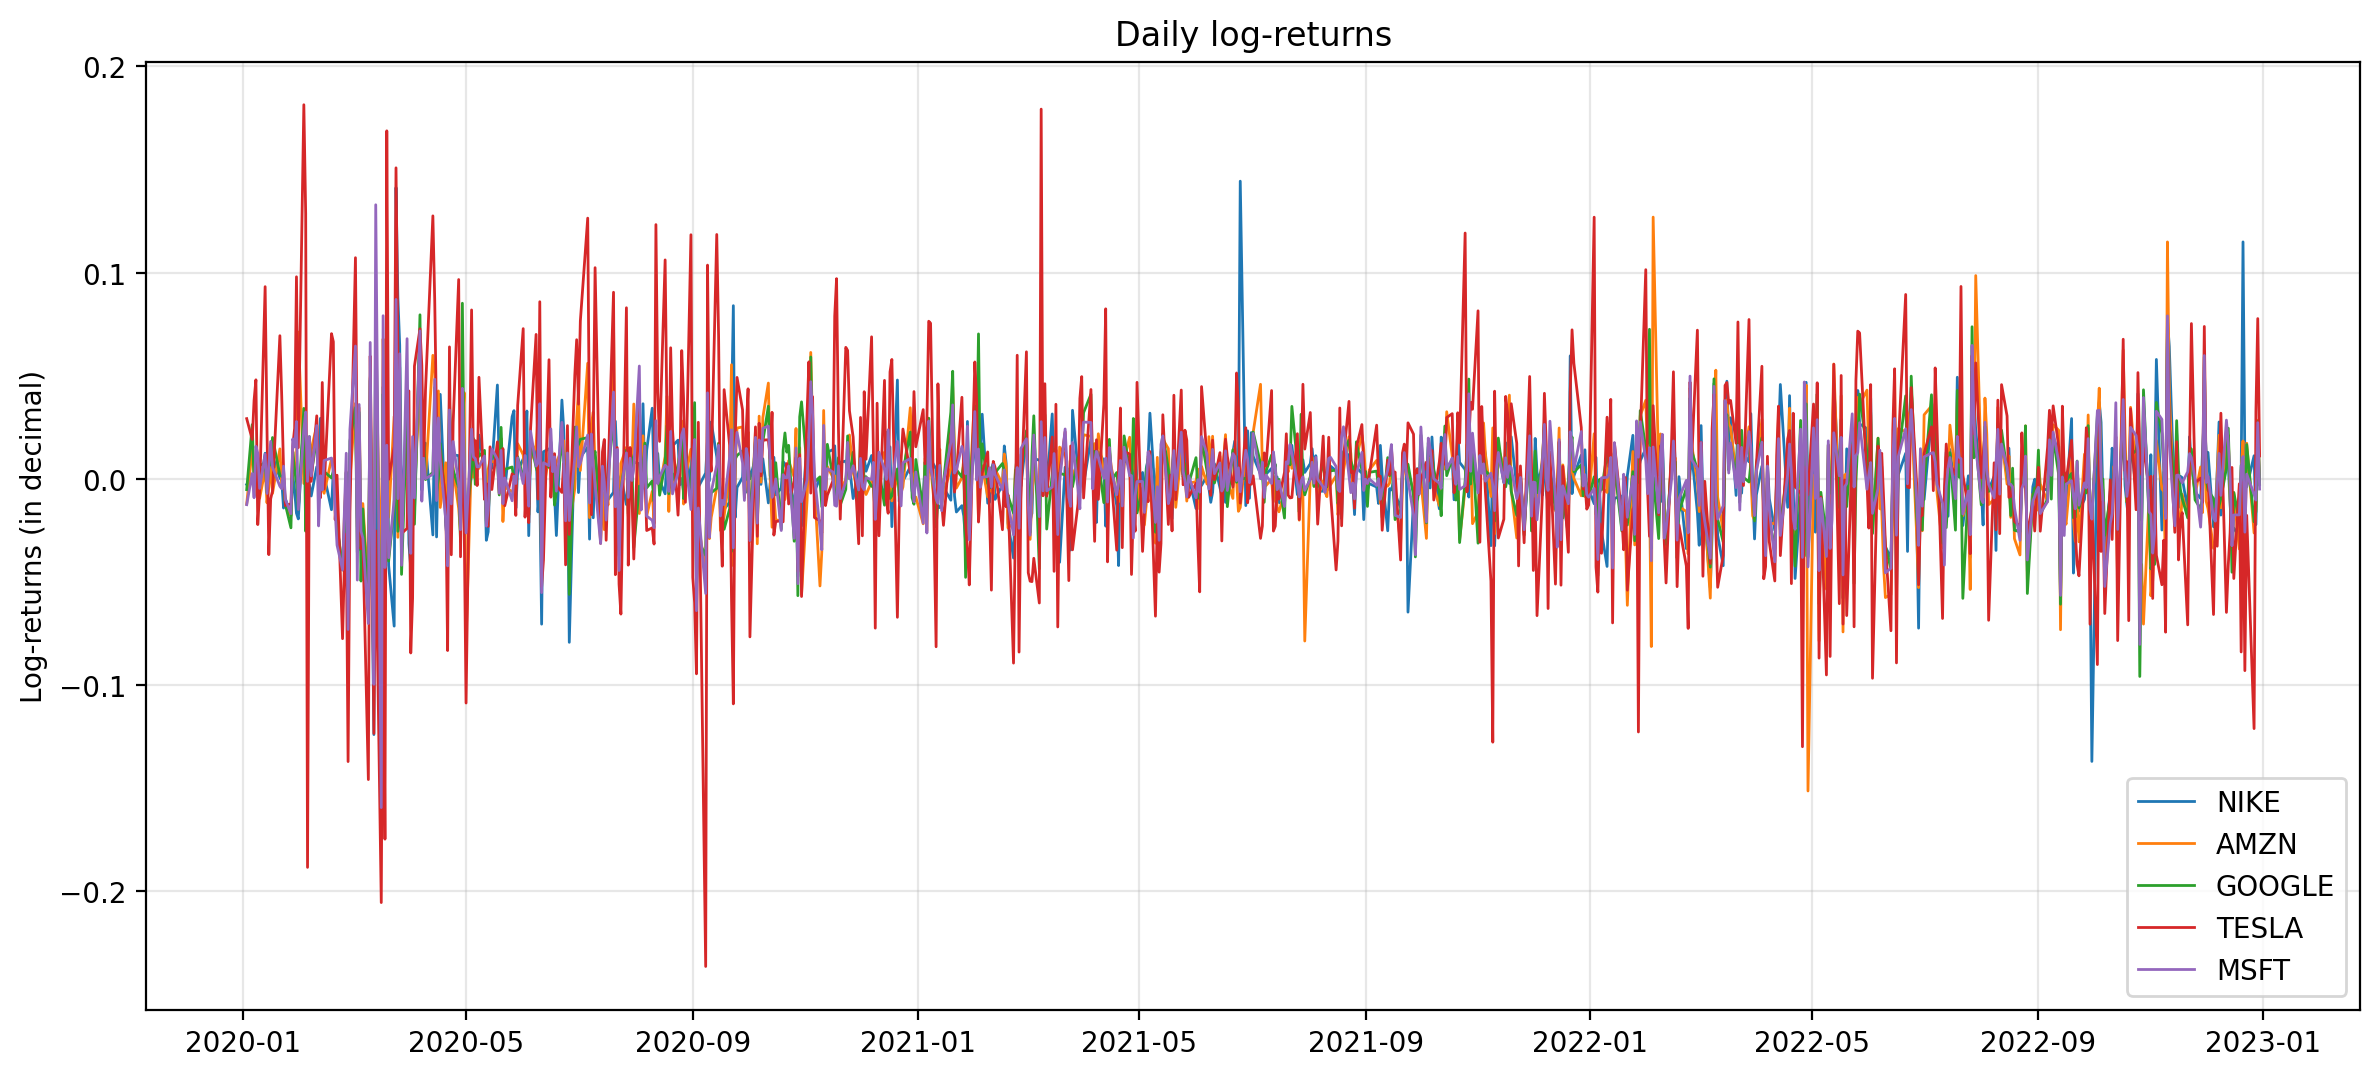
\includegraphics[width=0.9\textwidth]{outputs/figures/02_asset_returns.png}
\caption{Daily log-returns}
\label{fig:returns}
\end{figure}

Figure \ref{fig:returns} highlights volatility clustering and fat-tailed behavior, especially for Tesla. This suggests that optimization results will depend critically on both covariance and higher-moment features of the sample.

\begin{figure}[H]
\centering
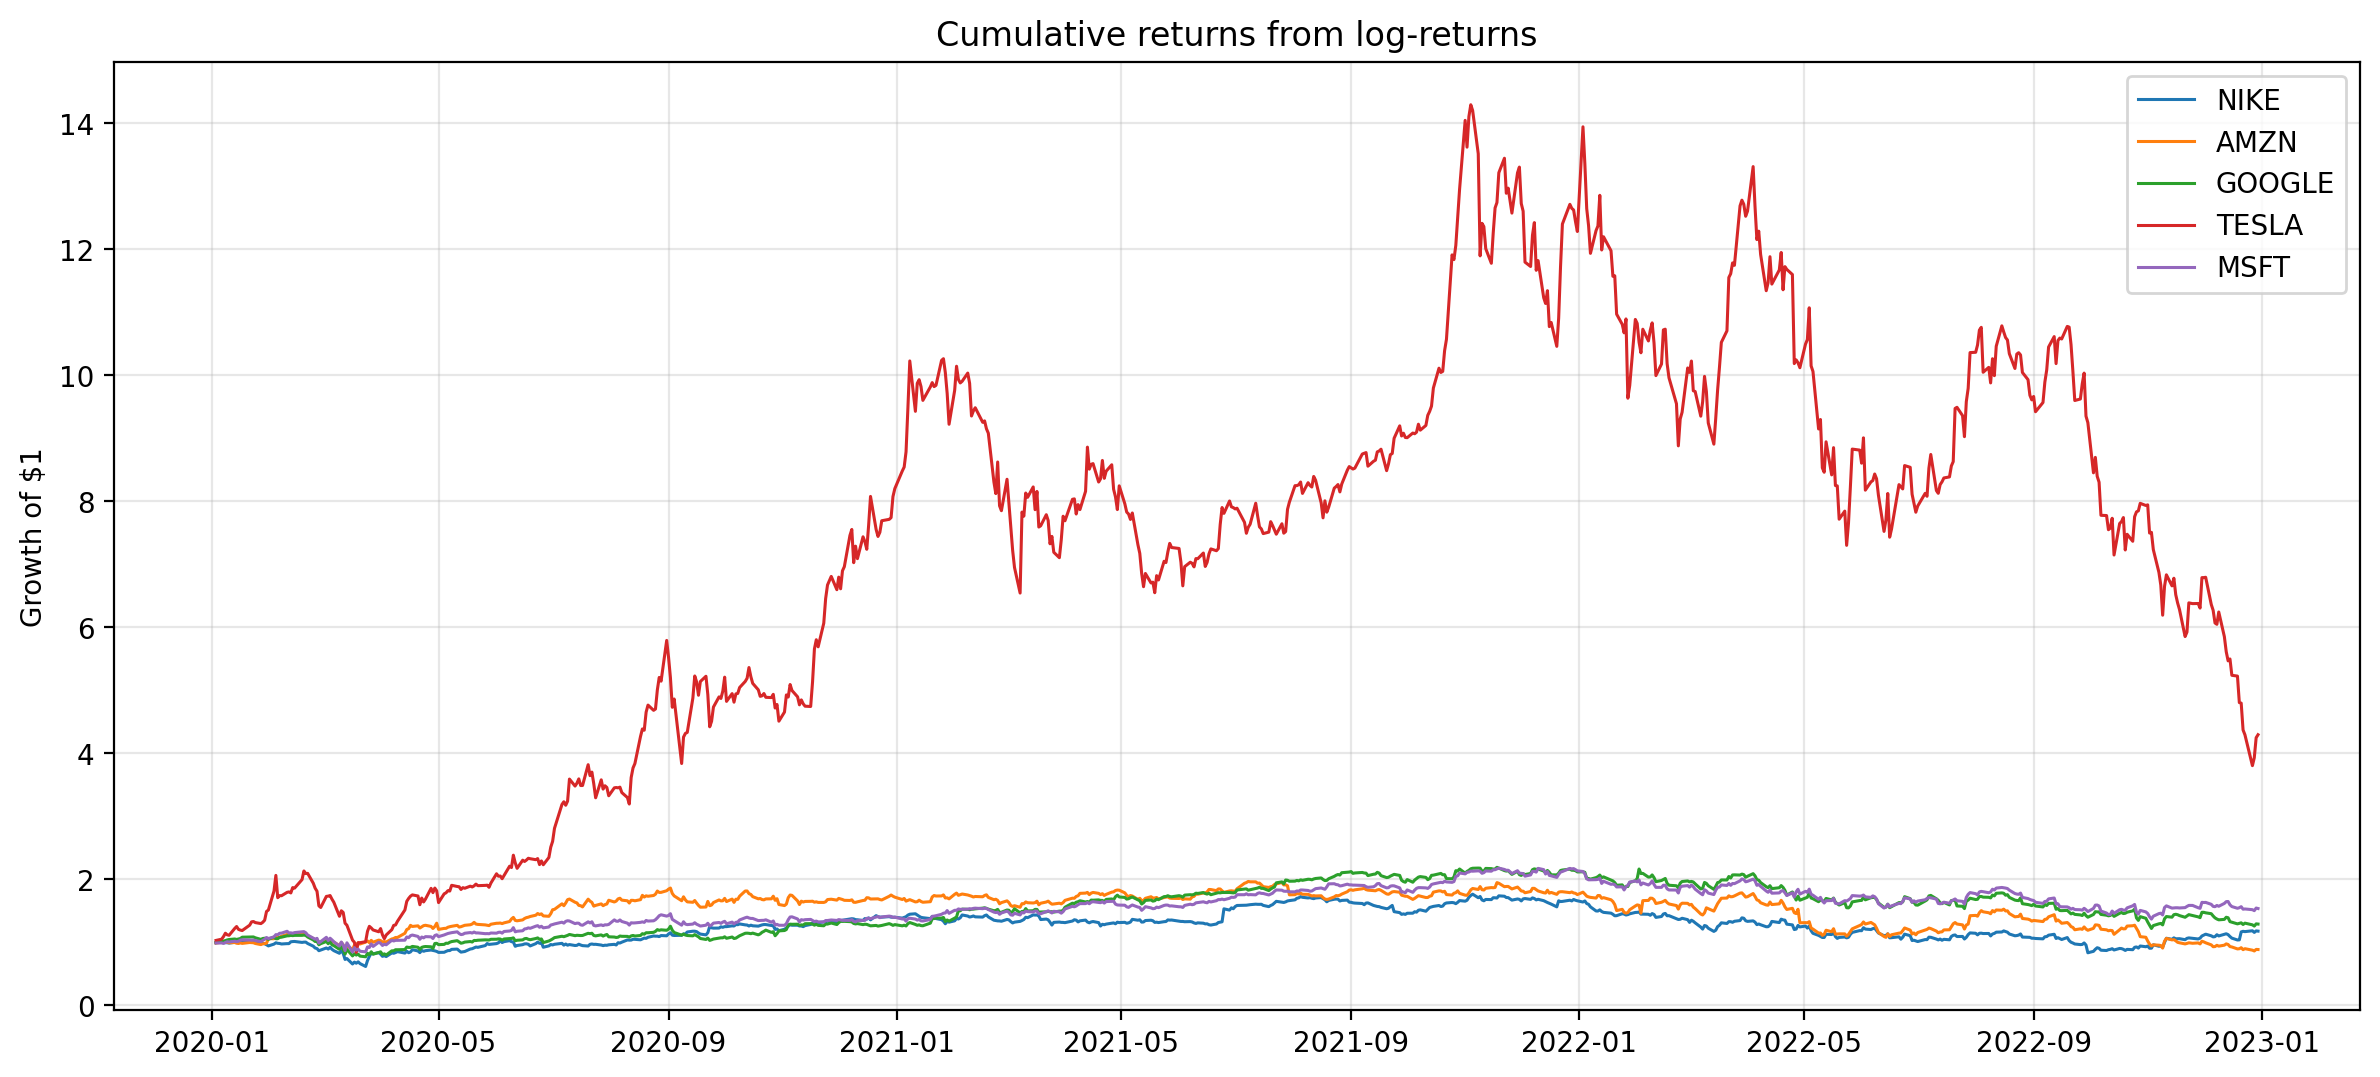
\includegraphics[width=0.9\textwidth]{outputs/figures/03_cumulative_returns.png}
\caption{Cumulative returns from log-returns}
\label{fig:cum_returns}
\end{figure}

Figure \ref{fig:cum_returns} shows the growth of \$1 invested in each asset. Tesla dominates cumulative performance over large parts of the sample, which later helps explain why return-seeking optimization rules assign it strong weight.

\subsection{Asset Summary Statistics}

Table \ref{tab:asset_summary} reports descriptive statistics for the five return series. Tesla has the highest average daily return, but it also has by far the largest standard deviation, confirming that its strong performance comes with substantially higher volatility. Google and Microsoft exhibit lower dispersion, while Amazon has a slightly negative average daily return over the sample.

\begin{table}[H]
\centering
\caption{Asset summary statistics}
\label{tab:asset_summary}
\small
\begin{tabular}{lrrrrr}
\toprule
Statistic & NIKE & AMZN & GOOGLE & TESLA & MSFT \\
\midrule
Count     & 755.00000000 & 755.00000000 & 755.00000000 & 755.00000000 & 755.00000000 \\
Min       & -0.13711600 & -0.15143100 & -0.12372800 & -0.23651800 & -0.15945300 \\
Max       &  0.14435500 &  0.12694900 &  0.08837700 &  0.18144500 &  0.13292900 \\
Range     &  0.28147100 &  0.27838000 &  0.21210500 &  0.41796300 &  0.29238200 \\
Sum       &  0.16316300 & -0.12263900 &  0.25411700 &  1.45717400 &  0.42867500 \\
Median    &  0.00003700 &  0.00055400 &  0.00108700 &  0.00195100 &  0.00069900 \\
Mean      &  0.00021600 & -0.00016200 &  0.00033700 &  0.00193000 &  0.00056800 \\
Std. Dev. &  0.02376200 &  0.02463000 &  0.02177200 &  0.04548800 &  0.02192200 \\
Variance  &  0.00056500 &  0.00060700 &  0.00047400 &  0.00206900 &  0.00048100 \\
SE Mean   &  0.00086500 &  0.00089700 &  0.00079200 &  0.00165500 &  0.00079800 \\
Coef. Var.& 109.92874900 & -151.64568500 & 64.64677200 & 23.57050600 & 38.59581600 \\
Skewness  &  0.09889500 & -0.11023000 & -0.20798400 & -0.24394500 & -0.28261100 \\
Kurtosis  &  7.49750500 &  3.99811300 &  3.22091800 &  3.04619300 &  6.83211600 \\
\bottomrule
\end{tabular}
\end{table}

The large kurtosis values for Nike and Microsoft indicate heavier tails than a normal distribution, while Tesla combines the highest return with the highest risk. This is consistent with Figures \ref{fig:returns} and \ref{fig:cum_returns}.

\subsection{Correlation Structure}

Table \ref{tab:corr_matrix} shows the correlation matrix of daily log returns. The strongest correlation appears between Google and Microsoft, suggesting meaningful co-movement among large-cap technology firms. The weakest pairwise correlation is between Nike and Tesla, which suggests better diversification potential when those assets are combined.

\begin{table}[H]
\centering
\caption{Asset correlation matrix}
\label{tab:corr_matrix}
\small
\begin{tabular}{lrrrrr}
\toprule
 & NIKE & AMZN & GOOGLE & TESLA & MSFT \\
\midrule
NIKE   & 1.00000000 & 0.48213000 & 0.57655800 & 0.36322700 & 0.59122400 \\
AMZN   & 0.48213000 & 1.00000000 & 0.68205300 & 0.48059900 & 0.70288800 \\
GOOGLE & 0.57655800 & 0.68205300 & 1.00000000 & 0.46055700 & 0.83252800 \\
TESLA  & 0.36322700 & 0.48059900 & 0.46055700 & 1.00000000 & 0.51064700 \\
MSFT   & 0.59122400 & 0.70288800 & 0.83252800 & 0.51064700 & 1.00000000 \\
\bottomrule
\end{tabular}
\end{table}

This dependence structure helps explain why a risk-balanced allocation does not place excessive weight on highly correlated large-cap growth names, while still assigning a smaller weight to Tesla because of its substantially larger standalone volatility.

\subsection{Covariance Structure}

Table \ref{tab:cov_matrix} reports the covariance matrix. Tesla has the largest own variance, much larger than the other assets, which strongly influences optimization outcomes. In particular, risk-sensitive portfolios penalize Tesla more heavily despite its attractive mean return.

\begin{table}[H]
\centering
\caption{Asset covariance matrix}
\label{tab:cov_matrix}
\small
\begin{tabular}{lrrrrr}
\toprule
 & NIKE & AMZN & GOOGLE & TESLA & MSFT \\
\midrule
NIKE   & 0.00056465 & 0.00028240 & 0.00029821 & 0.00039260 & 0.00030767 \\
AMZN   & 0.00028240 & 0.00060662 & 0.00036620 & 0.00053837 & 0.00037961 \\
GOOGLE & 0.00029821 & 0.00036620 & 0.00047403 & 0.00045578 & 0.00039730 \\
TESLA  & 0.00039260 & 0.00053837 & 0.00045578 & 0.00206915 & 0.00050985 \\
MSFT   & 0.00030767 & 0.00037961 & 0.00039730 & 0.00050985 & 0.00048059 \\
\bottomrule
\end{tabular}
\end{table}

Together, Tables \ref{tab:corr_matrix} and \ref{tab:cov_matrix} provide the statistical foundation for all optimization routines in this study, since every portfolio’s risk is computed from the covariance matrix.

\section{Portfolio Theory and Optimization Framework}

\subsection{Portfolio Return and Risk}

For a portfolio with weight vector $w$, expected return vector $\mu$, and covariance matrix $\Sigma$, portfolio return and variance are defined as:
\begin{align}
\mu_p &= w^\top \mu, \\
\sigma_p^2 &= w^\top \Sigma w, \\
\sigma_p &= \sqrt{w^\top \Sigma w}.
\end{align}

\subsection{Minimum-Variance Portfolio}

The global minimum-variance portfolio solves
\begin{equation}
\min_w \quad w^\top \Sigma w \quad \text{s.t.} \quad \mathbf{1}^\top w = 1.
\end{equation}

This portfolio minimizes total risk without directly targeting return.

\subsection{Maximum-Return Portfolio with Box Constraints}

The maximum-return portfolio solves
\begin{equation}
\max_w \quad w^\top \mu
\end{equation}
subject to
\begin{equation}
\mathbf{1}^\top w = 1, \qquad 0 \leq w_i \leq 0.25.
\end{equation}

The box constraints ensure that no single asset receives more than 25\% of total capital.

\subsection{Dollar-Neutral Portfolio}

The dollar-neutral strategy approximately satisfies
\begin{align}
\sum_{i=1}^n w_i &\approx 0, \\
-0.25 \leq w_i &\leq 0.25,
\end{align}
with a maximum of three active positions. The implementation searches for weights that match target mean and target standard deviation:
\begin{equation}
\min_w \left[ (\mu_p - \mu^\star)^2 + (\sigma_p - \sigma^\star)^2 \right].
\end{equation}

\subsection{Risk-Parity Portfolio}

Risk parity equalizes percentage contributions to total portfolio variance. The contribution of asset $i$ is
\begin{equation}
RC_i = \frac{w_i (\Sigma w)_i}{w^\top \Sigma w}.
\end{equation}
The optimization seeks
\begin{equation}
\min_w \sum_{i=1}^n \left(RC_i - \frac{1}{n}\right)^2
\end{equation}
subject to long-only and full-investment constraints.

\subsection{Tangency Portfolio}

The tangency portfolio maximizes the Sharpe ratio:
\begin{equation}
\max_w \quad \frac{w^\top \mu - r_f}{\sqrt{w^\top \Sigma w}}
\end{equation}
subject to
\begin{equation}
\mathbf{1}^\top w = 1, \qquad w_i \geq 0.
\end{equation}

Under the unconstrained formulation, the tangency weights take the form
\begin{equation}
w_T \propto \Sigma^{-1}(\mu - r_f \mathbf{1}),
\end{equation}
with normalization chosen so the weights sum to one. In the present constrained implementation, the optimizer selects the long-only portfolio with the highest risk-adjusted return.

\section{Efficient Frontier and Sharpe Ratio Geometry}

The efficient frontier is approximated using simulated long-only portfolios. For each random portfolio, the code computes the pair $(\sigma_p,\mu_p)$ and plots the feasible cloud.

\begin{figure}[H]
\centering
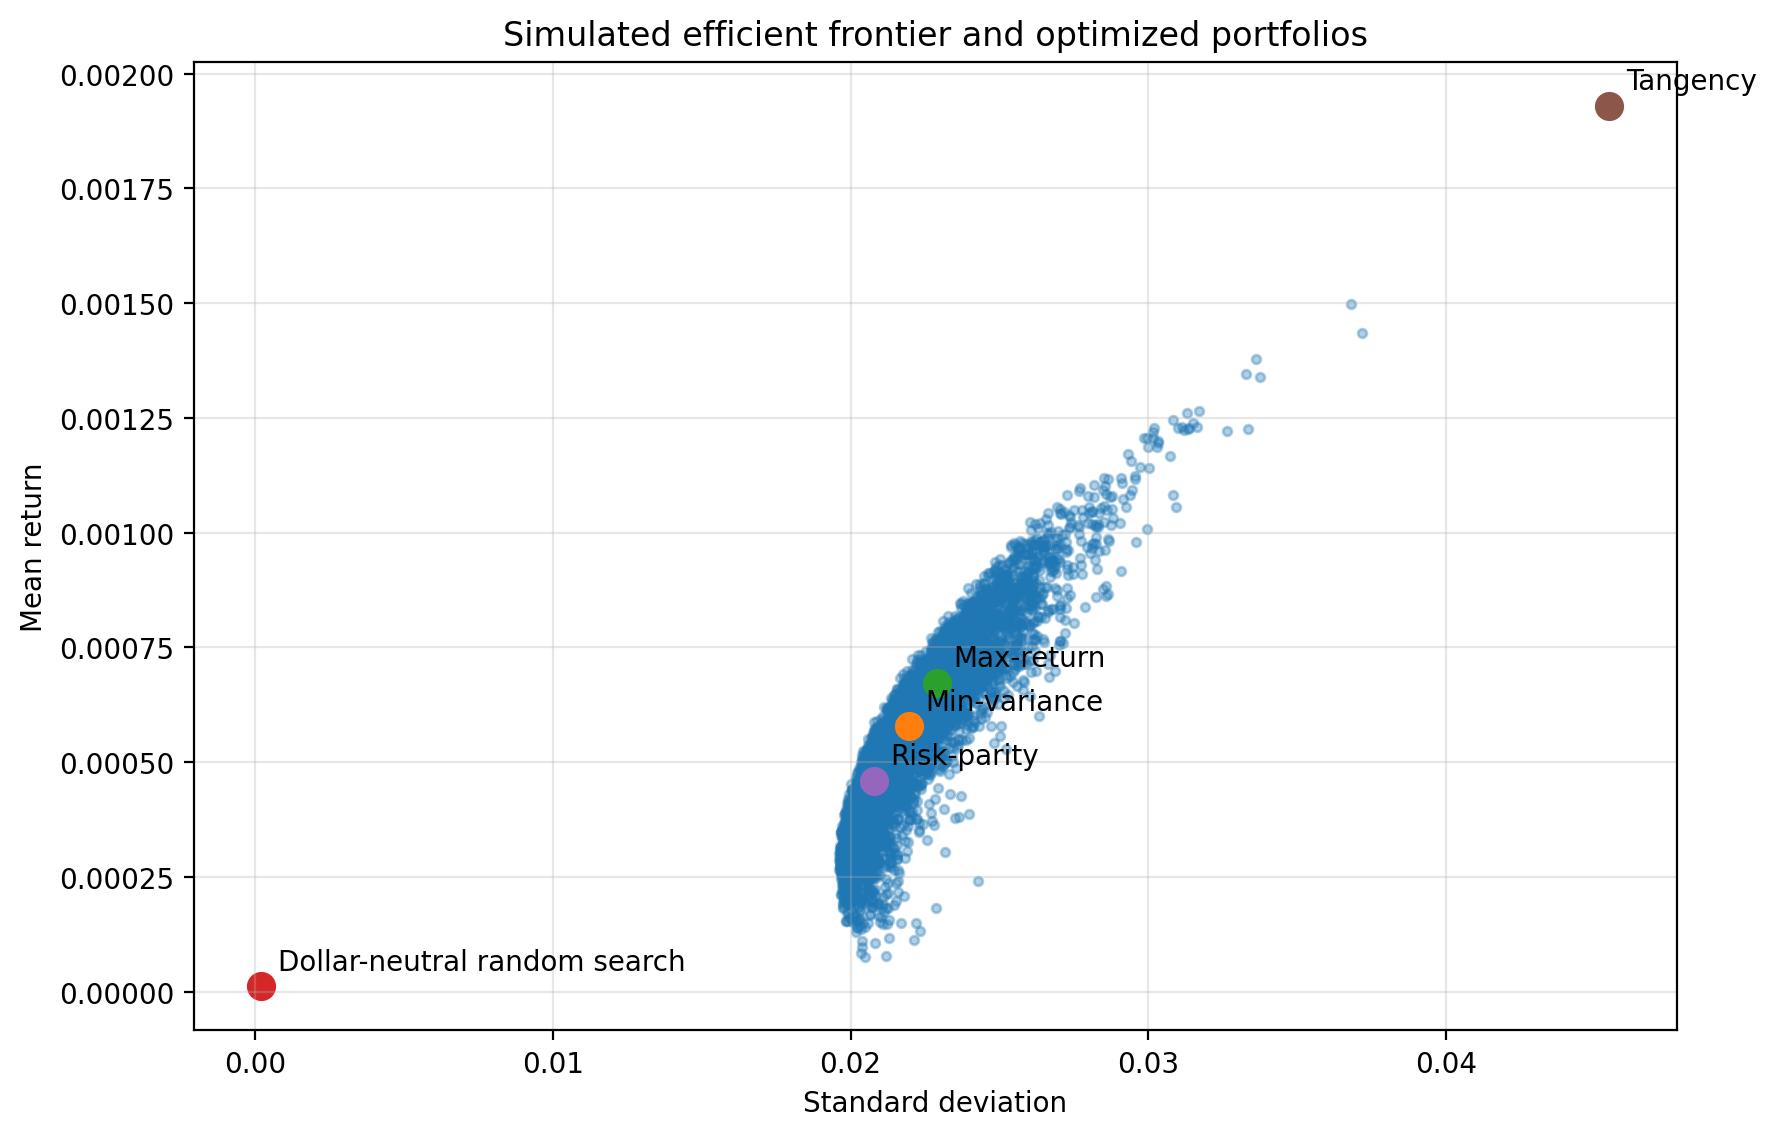
\includegraphics[width=0.9\textwidth]{outputs/figures/41_efficient_frontier.png}
\caption{Simulated efficient frontier and optimized portfolios}
\label{fig:frontier}
\end{figure}

Figure \ref{fig:frontier} shows the simulated opportunity set together with the optimized portfolios. The tangency portfolio appears at the upper-right boundary because it delivers the highest average return, while the dollar-neutral portfolio lies near the origin due to its near-zero net exposure.

Sharpe ratio iso-lines are defined by
\begin{equation}
\mu_p = r_f + S \sigma_p,
\end{equation}
where $S$ is a constant Sharpe ratio. These lines are straight in mean-standard deviation space. The tangency portfolio is the portfolio at which the highest attainable Sharpe iso-line touches the efficient frontier.

\section{Utility Maximization and Indifference Curves}

Investor preferences are modeled with quadratic utility:
\begin{equation}
U = \mu_p - \frac{A}{2}\sigma_p^2,
\end{equation}
where $A>0$ is the coefficient of risk aversion.

For a fixed level of utility $U_0$, the indifference curve is
\begin{equation}
\mu_p = U_0 + \frac{A}{2}\sigma_p^2.
\end{equation}

Thus, more risk-averse investors require greater expected return to accept the same increase in risk.

\begin{figure}[H]
\centering
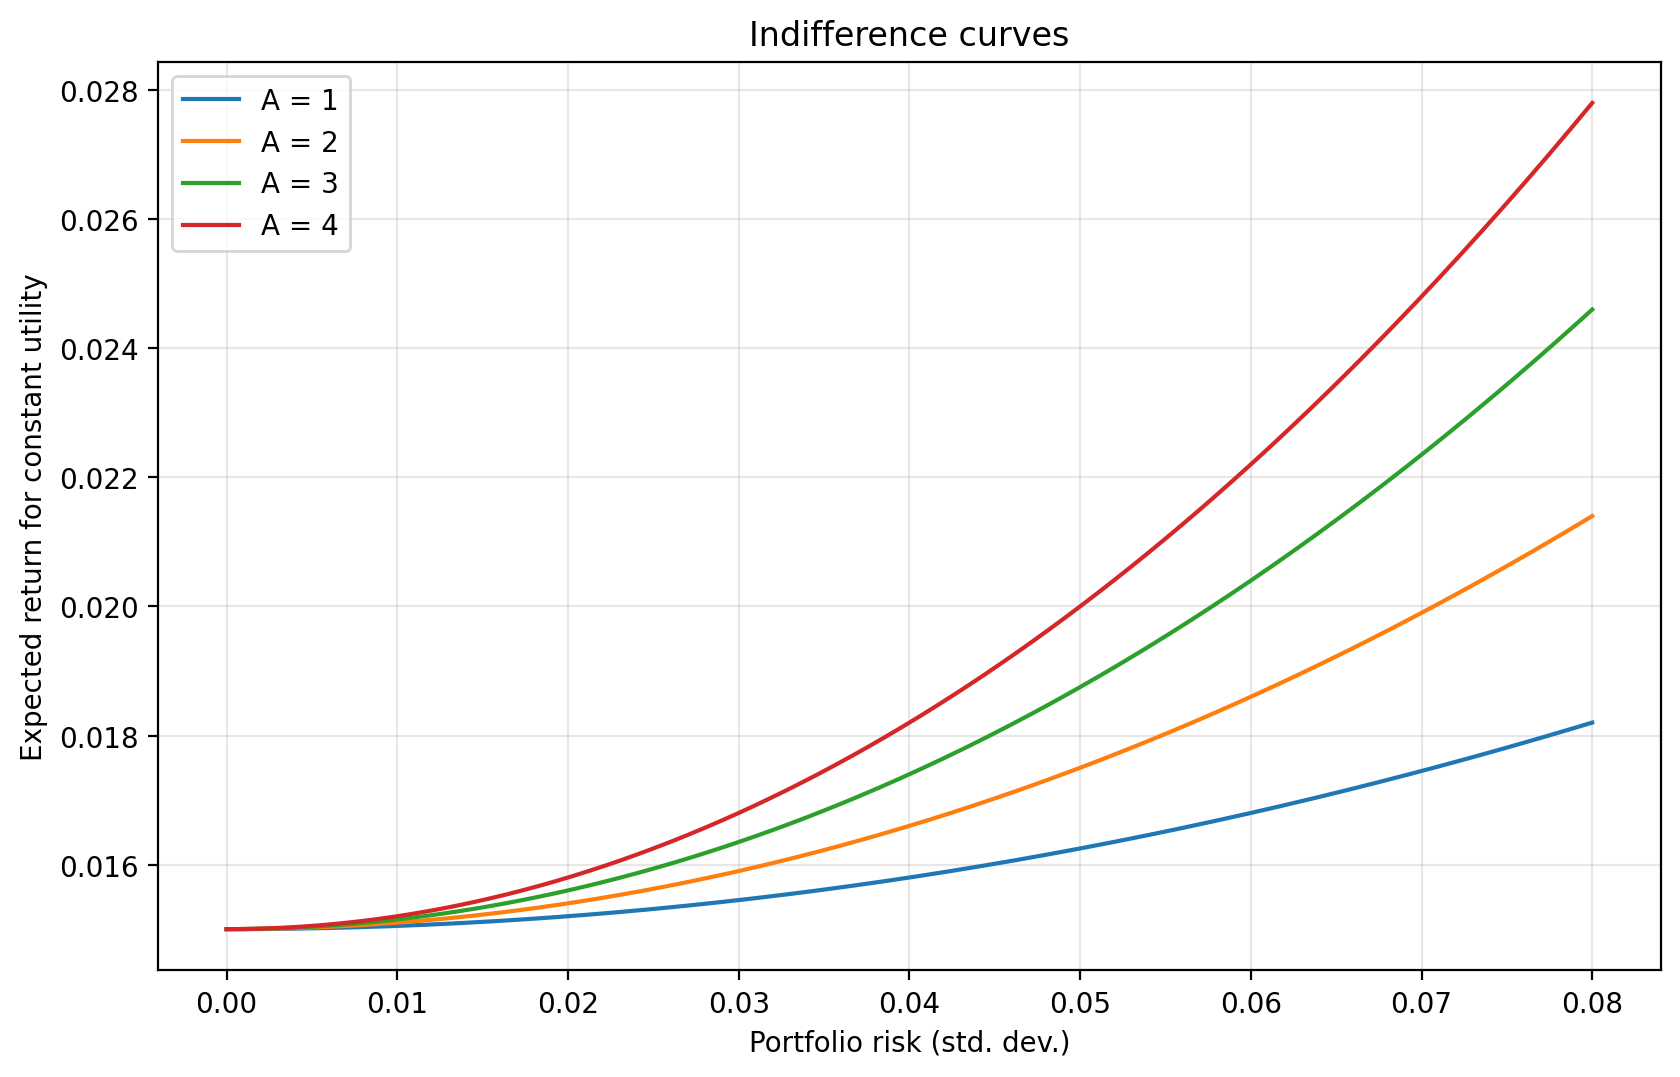
\includegraphics[width=0.9\textwidth]{outputs/figures/42_indifference_curves.png}
\caption{Investor indifference curves for different levels of risk aversion}
\label{fig:indifference}
\end{figure}

Figure \ref{fig:indifference} illustrates this trade-off. Curves associated with larger $A$ are steeper, meaning that highly risk-averse investors demand substantially higher expected return for the same level of volatility.

The investor’s optimal risky portfolio is the point at which the highest attainable indifference curve is tangent to the efficient frontier. At the optimum, the slope of the frontier equals the slope of the indifference curve:
\begin{equation}
\frac{d\mu_p}{d\sigma_p} = A\sigma_p.
\end{equation}

This condition links the geometry of the frontier with the economic interpretation of risk aversion.

\section{Portfolio Results}

\subsection{Portfolio Weight Allocations}

Table \ref{tab:weights} reports the optimized asset allocations across the five portfolio construction rules.

\begin{table}[H]
\centering
\caption{Portfolio weights}
\label{tab:weights}
\small
\begin{tabular}{lrrrrr}
\toprule
Asset & Min-variance & Max-return & Dollar-neutral & Risk-parity & Tangency \\
\midrule
NIKE   & 0.20000000 & 0.18659067 &  0.00000000 & 0.23316256 & 0.00000000 \\
AMZN   & 0.20000000 & 0.17223156 & -0.00531527 & 0.20557259 & 0.00000000 \\
GOOGLE & 0.20000000 & 0.19118093 &  0.00000000 & 0.22034040 & 0.00000000 \\
TESLA  & 0.20000000 & 0.25000000 &  0.00531527 & 0.12782408 & 1.00000000 \\
MSFT   & 0.20000000 & 0.19999684 &  0.00000000 & 0.21310037 & 0.00000000 \\
\bottomrule
\end{tabular}
\end{table}

The weight patterns highlight the economic logic of each optimizer. The minimum-variance portfolio is equally weighted in the reported output, indicating that under the estimated covariance structure and imposed constraints, the optimizer settles on a symmetric allocation. The maximum-return portfolio pushes Tesla to its upper bound of 25\%, reflecting Tesla’s dominant mean return in Table \ref{tab:asset_summary}. The dollar-neutral solution uses a very small short position in Amazon offset by a small long position in Tesla, producing a nearly market-neutral payoff. Risk parity assigns the smallest weight to Tesla because its standalone variance is much larger than that of the other assets. Finally, the tangency portfolio fully concentrates in Tesla, indicating that Tesla delivers the strongest return-to-risk trade-off under the implemented Sharpe-ratio objective.

\begin{figure}[H]
\centering
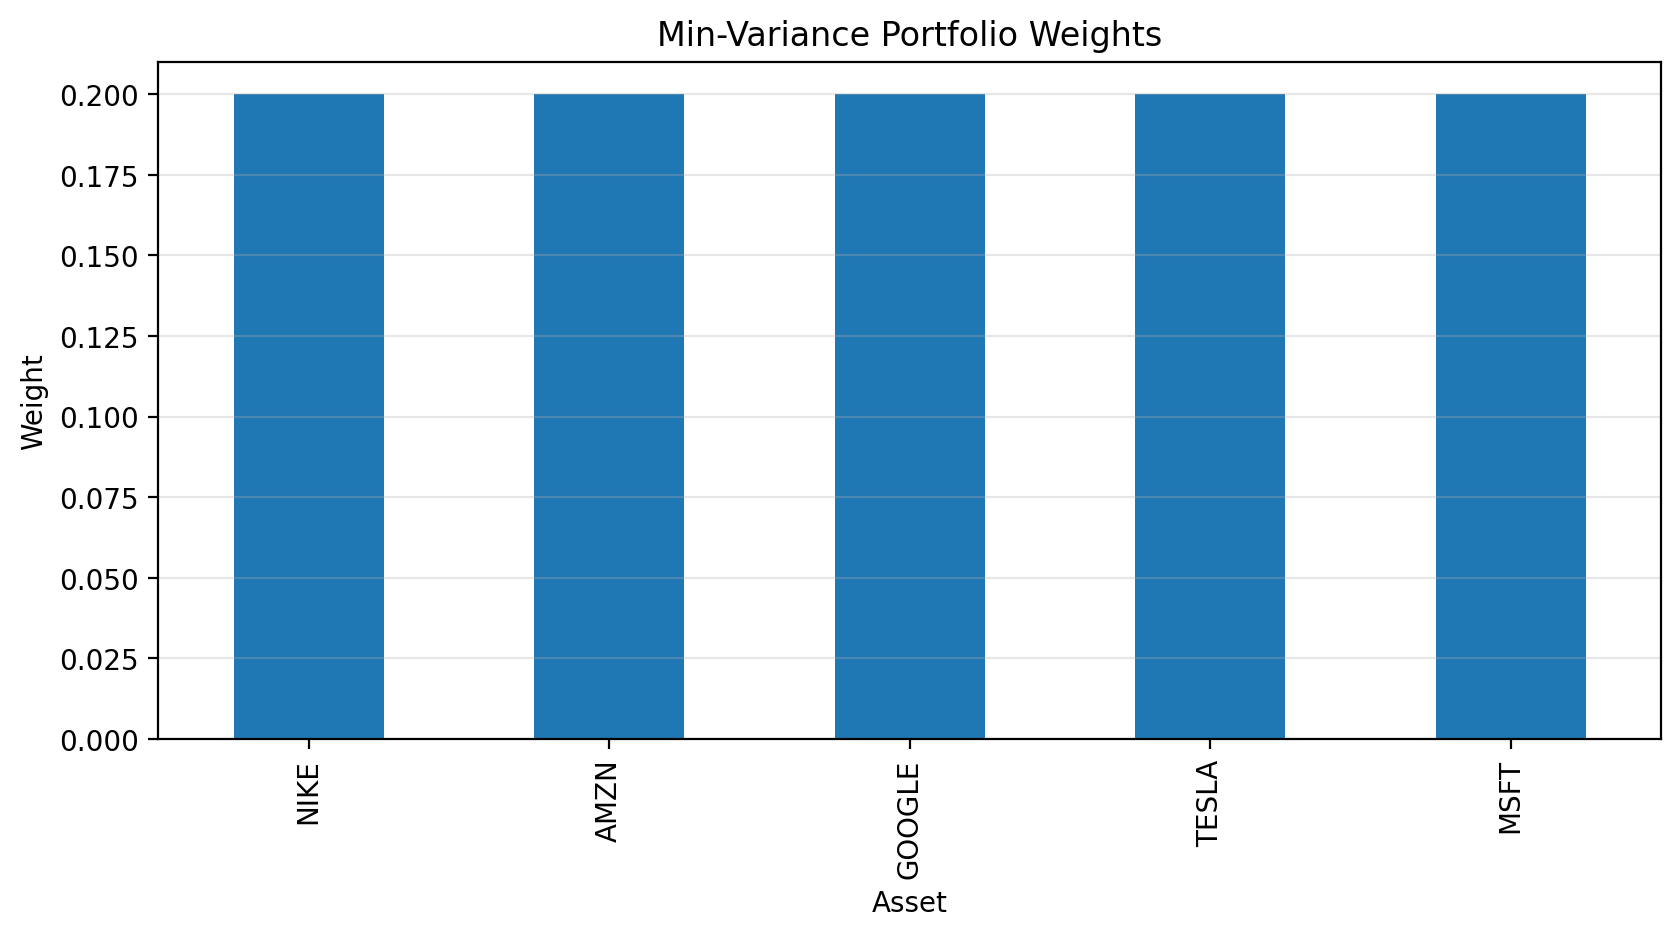
\includegraphics[width=0.72\textwidth]{outputs/figures/11_min_variance_weights.png}
\caption{Minimum-variance portfolio weights}
\label{fig:minvar_weights}
\end{figure}

\begin{figure}[H]
\centering
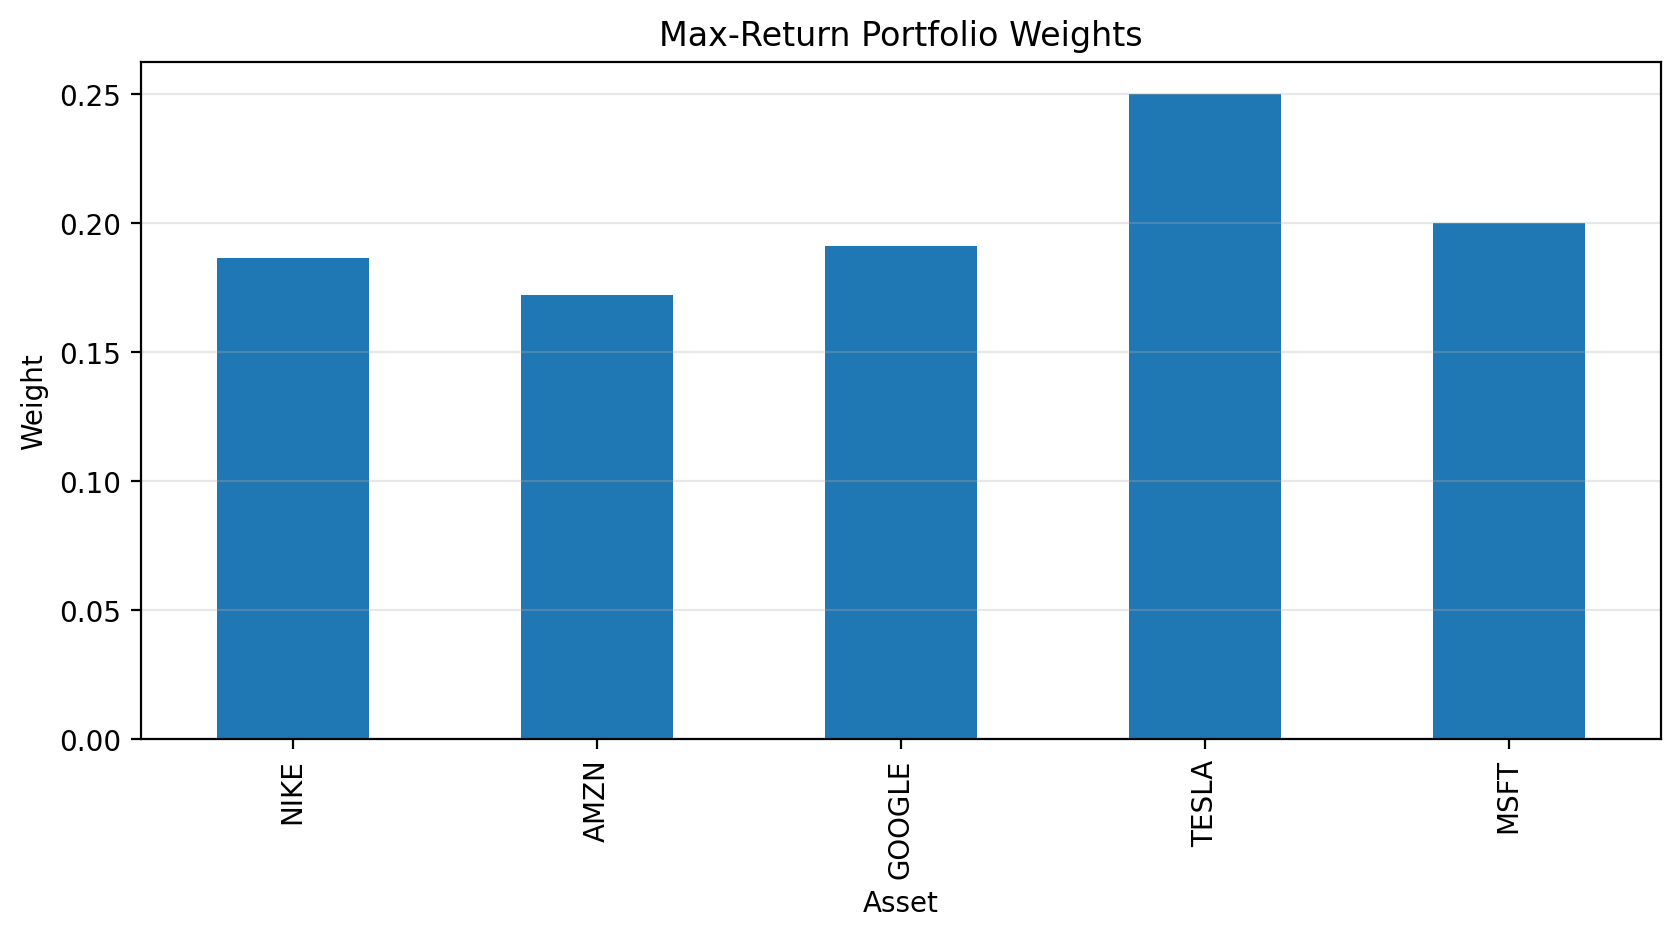
\includegraphics[width=0.72\textwidth]{outputs/figures/12_max_return_weights.png}
\caption{Maximum-return portfolio weights}
\label{fig:maxret_weights}
\end{figure}

\begin{figure}[H]
\centering
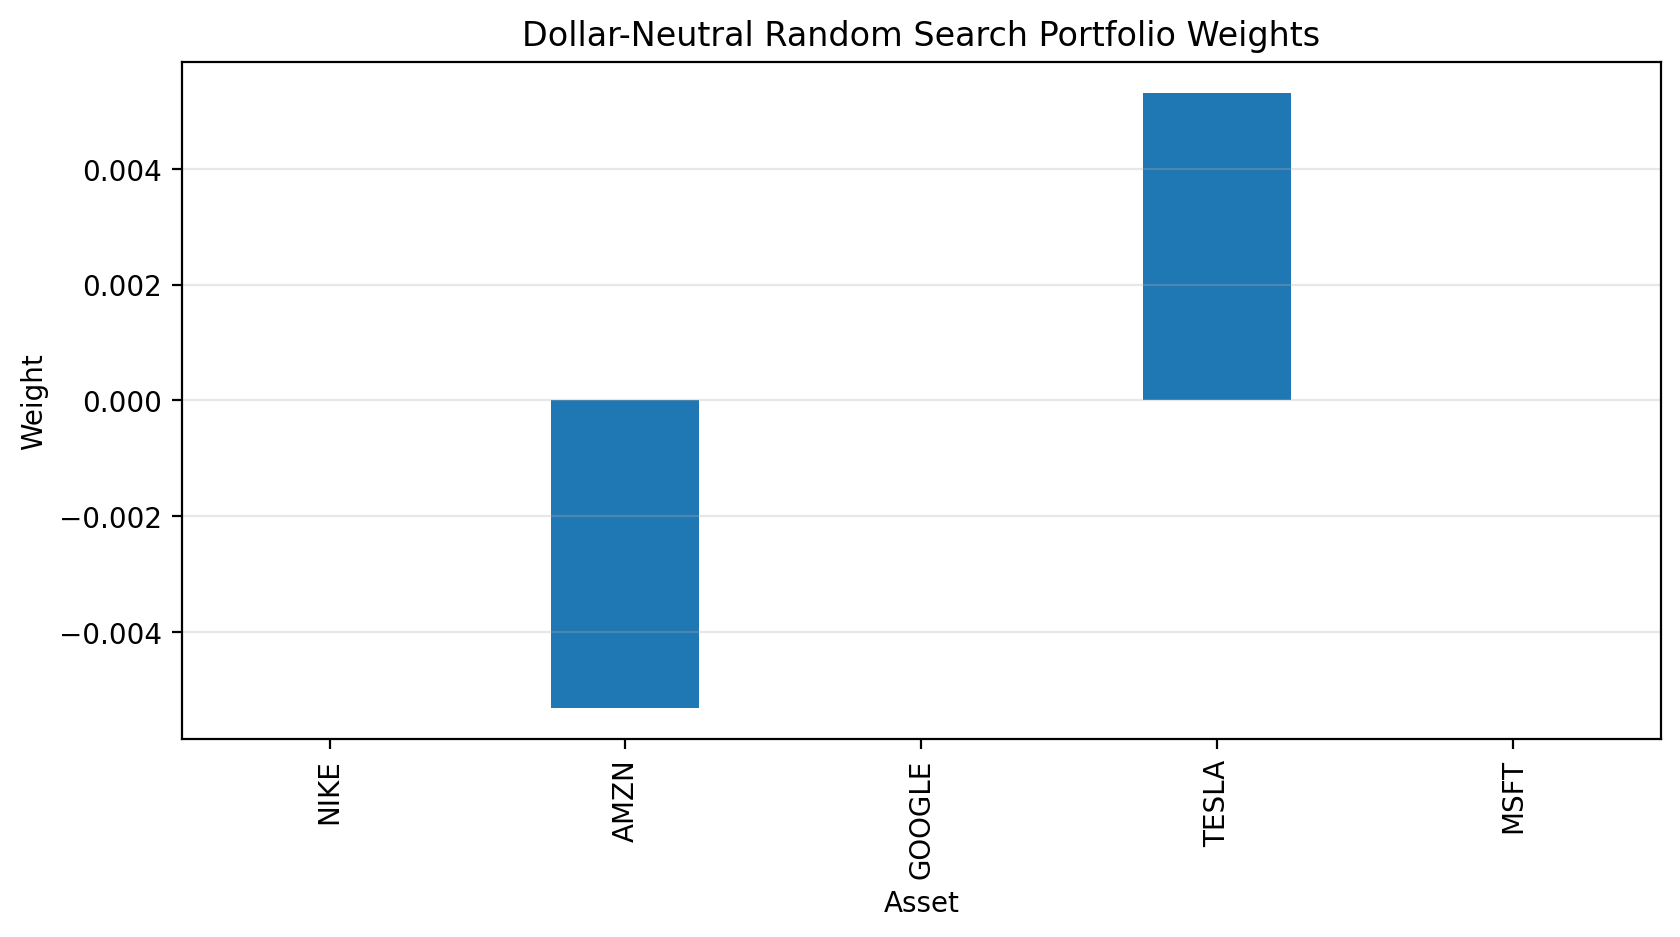
\includegraphics[width=0.72\textwidth]{outputs/figures/13_dollar_neutral_random_search_weights.png}
\caption{Dollar-neutral random search portfolio weights}
\label{fig:dn_weights}
\end{figure}

\begin{figure}[H]
\centering
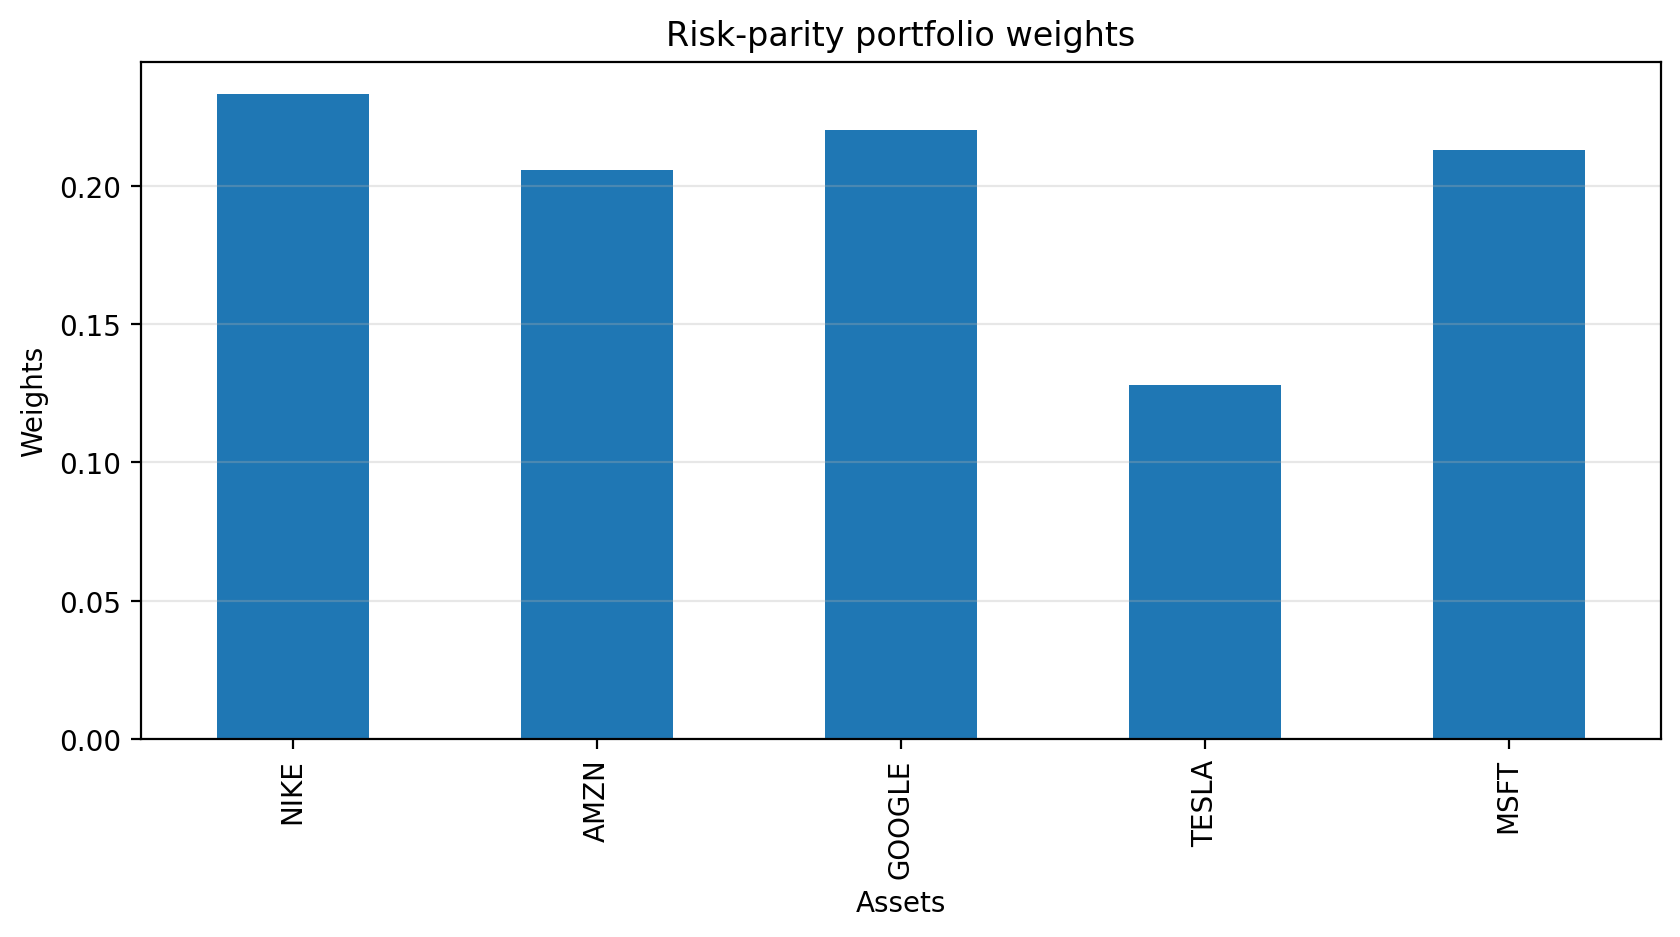
\includegraphics[width=0.72\textwidth]{outputs/figures/14_risk_parity_weights.png}
\caption{Risk-parity portfolio weights}
\label{fig:rp_weights}
\end{figure}

\begin{figure}[H]
\centering
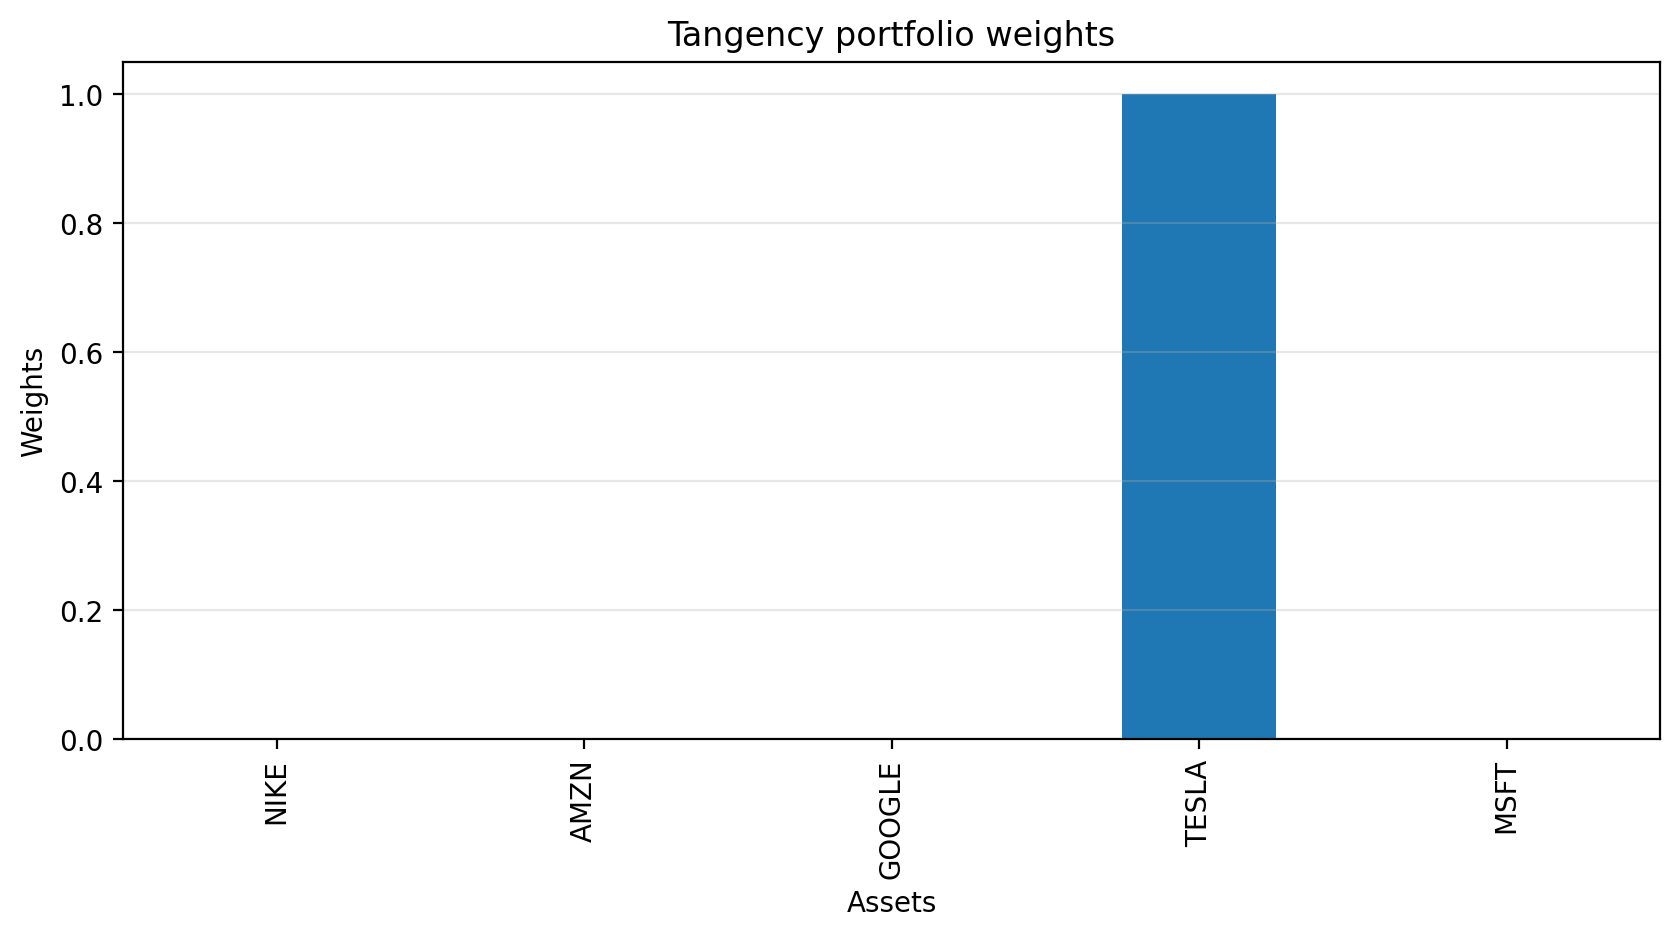
\includegraphics[width=0.72\textwidth]{outputs/figures/15_tangency_weights.png}
\caption{Tangency portfolio weights}
\label{fig:tangency_weights}
\end{figure}

Figures \ref{fig:minvar_weights}--\ref{fig:tangency_weights} visually confirm the allocation logic summarized in Table \ref{tab:weights}. The tangency portfolio is extreme by construction, while risk parity is the most balanced among the long-only optimized allocations.

\subsection{Portfolio Summary Statistics}

Figure \ref{fig:risk_return} compares the optimized portfolios in mean-standard deviation space, and Table \ref{tab:portfolio_summary} summarizes their key statistics.

\begin{figure}[H]
\centering
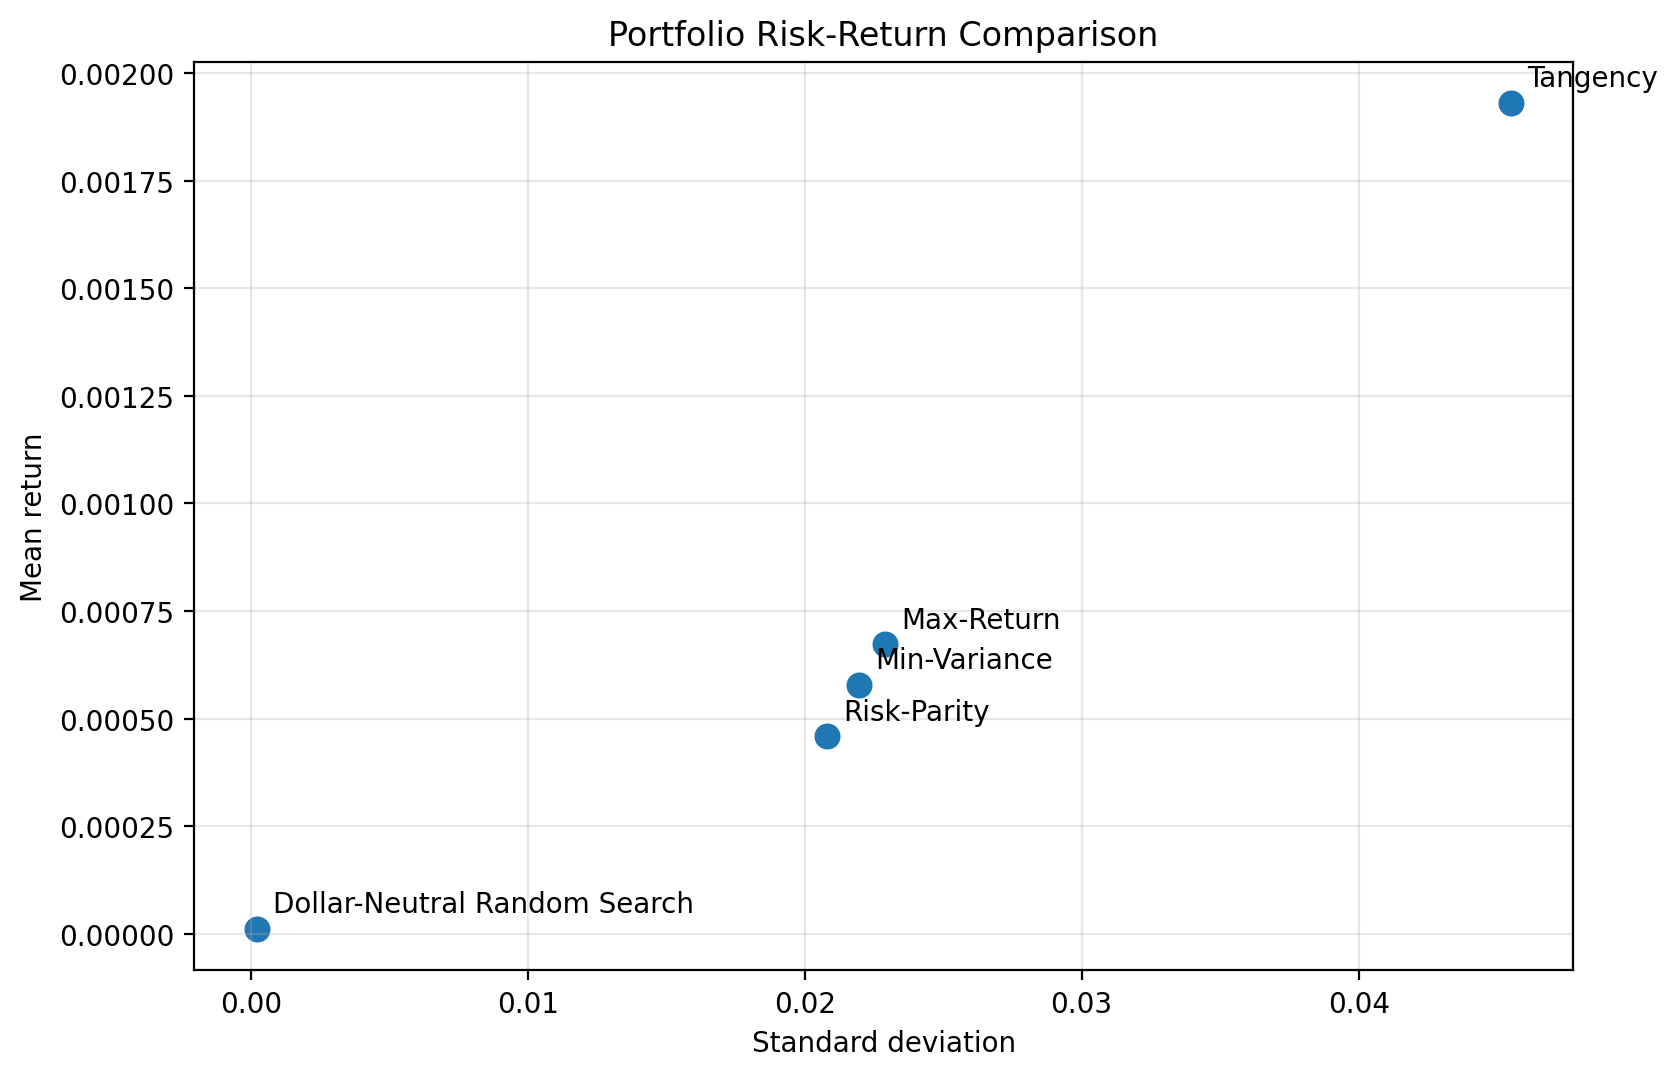
\includegraphics[width=0.9\textwidth]{outputs/figures/40_portfolio_risk_return_comparison.png}
\caption{Portfolio risk-return comparison}
\label{fig:risk_return}
\end{figure}

\begin{table}[H]
\centering
\caption{Portfolio summary statistics}
\label{tab:portfolio_summary}
\small
\begin{tabular}{lrrrrr}
\toprule
Portfolio & Mean & Std. Dev. & Variance & Daily Sharpe & Annualized Sharpe \\
\midrule
Min-variance & 0.00057771 & 0.02195455 & 0.00048200 & -0.88464624 & -14.04304113 \\
Max-return & 0.00067275 & 0.02289264 & 0.00052407 & -0.84420390 & -13.40161009 \\
Dollar-neutral random search & 0.00001147 & 0.00021252 & 0.00000005 & -94.05718427 & -1493.11241055 \\
Risk-parity & 0.00045877 & 0.02078788 & 0.00043214 & -0.94004034 & -14.92218408 \\
Tangency & 0.00192995 & 0.04548788 & 0.00206915 & -0.39724531 & -6.30598379 \\
\bottomrule
\end{tabular}
\end{table}

Table \ref{tab:portfolio_summary} confirms the visual pattern in Figure \ref{fig:risk_return}. The tangency portfolio has the highest average return but also the highest volatility. The risk-parity portfolio has the lowest standard deviation among the long-only diversified solutions, while the dollar-neutral strategy has near-zero mean and near-zero volatility, as intended by construction. The minimum-variance and maximum-return portfolios are relatively close in risk, but the maximum-return portfolio delivers a slightly larger average return.

\begin{table}[H]
\centering
\caption{Interpretation summary of optimization outcomes}
\label{tab:interpretation_summary}
\small
\begin{tabular}{lp{0.72\linewidth}}
\toprule
Portfolio & Main interpretation \\
\midrule
Min-variance & Delivers moderate return with controlled volatility; reported solution is equally weighted in the current implementation. \\
Max-return & Tilts toward the highest-return asset subject to the box constraint, which pushes Tesla to the maximum allowed weight. \\
Dollar-neutral & Constructs a near-zero exposure strategy with offsetting long and short positions, targeting very low risk and near-zero average return. \\
Risk-parity & Allocates capital so that no single asset dominates total portfolio risk; Tesla receives the smallest weight because of its large variance. \\
Tangency & Maximizes return per unit of risk and becomes fully concentrated in Tesla under the implemented Sharpe-ratio criterion. \\
\bottomrule
\end{tabular}
\end{table}

Table \ref{tab:interpretation_summary} summarizes the economic role of each optimization rule and provides a concise interpretation of the numerical and graphical evidence.

\section{Return Distributions}

The distributional plots provide an additional layer of interpretation beyond means and variances. The minimum-variance and risk-parity portfolios have relatively tight and centered densities, indicating stable return behavior. By contrast, the tangency portfolio’s histogram is visibly wider, reflecting its full concentration in Tesla and the resulting exposure to large positive and negative daily moves.

\begin{figure}[H]
\centering
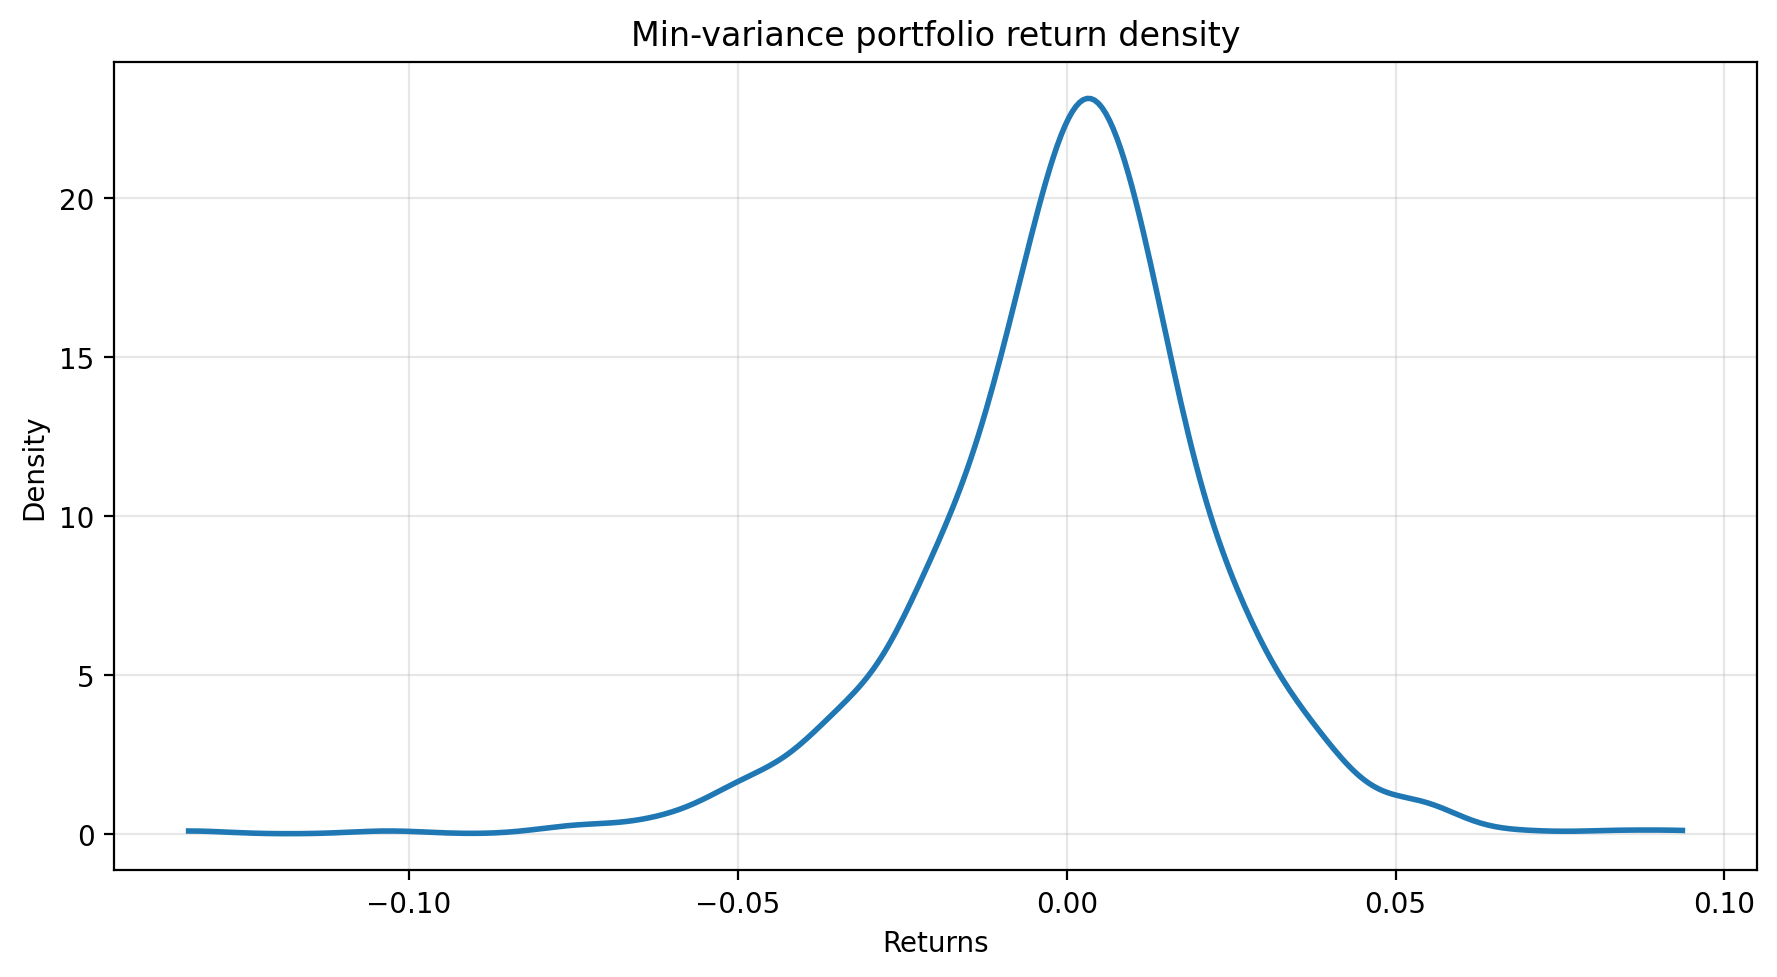
\includegraphics[width=0.8\textwidth]{outputs/figures/31_min_variance_density.png}
\caption{Minimum-variance portfolio return density}
\label{fig:minvar_density}
\end{figure}

\begin{figure}[H]
\centering
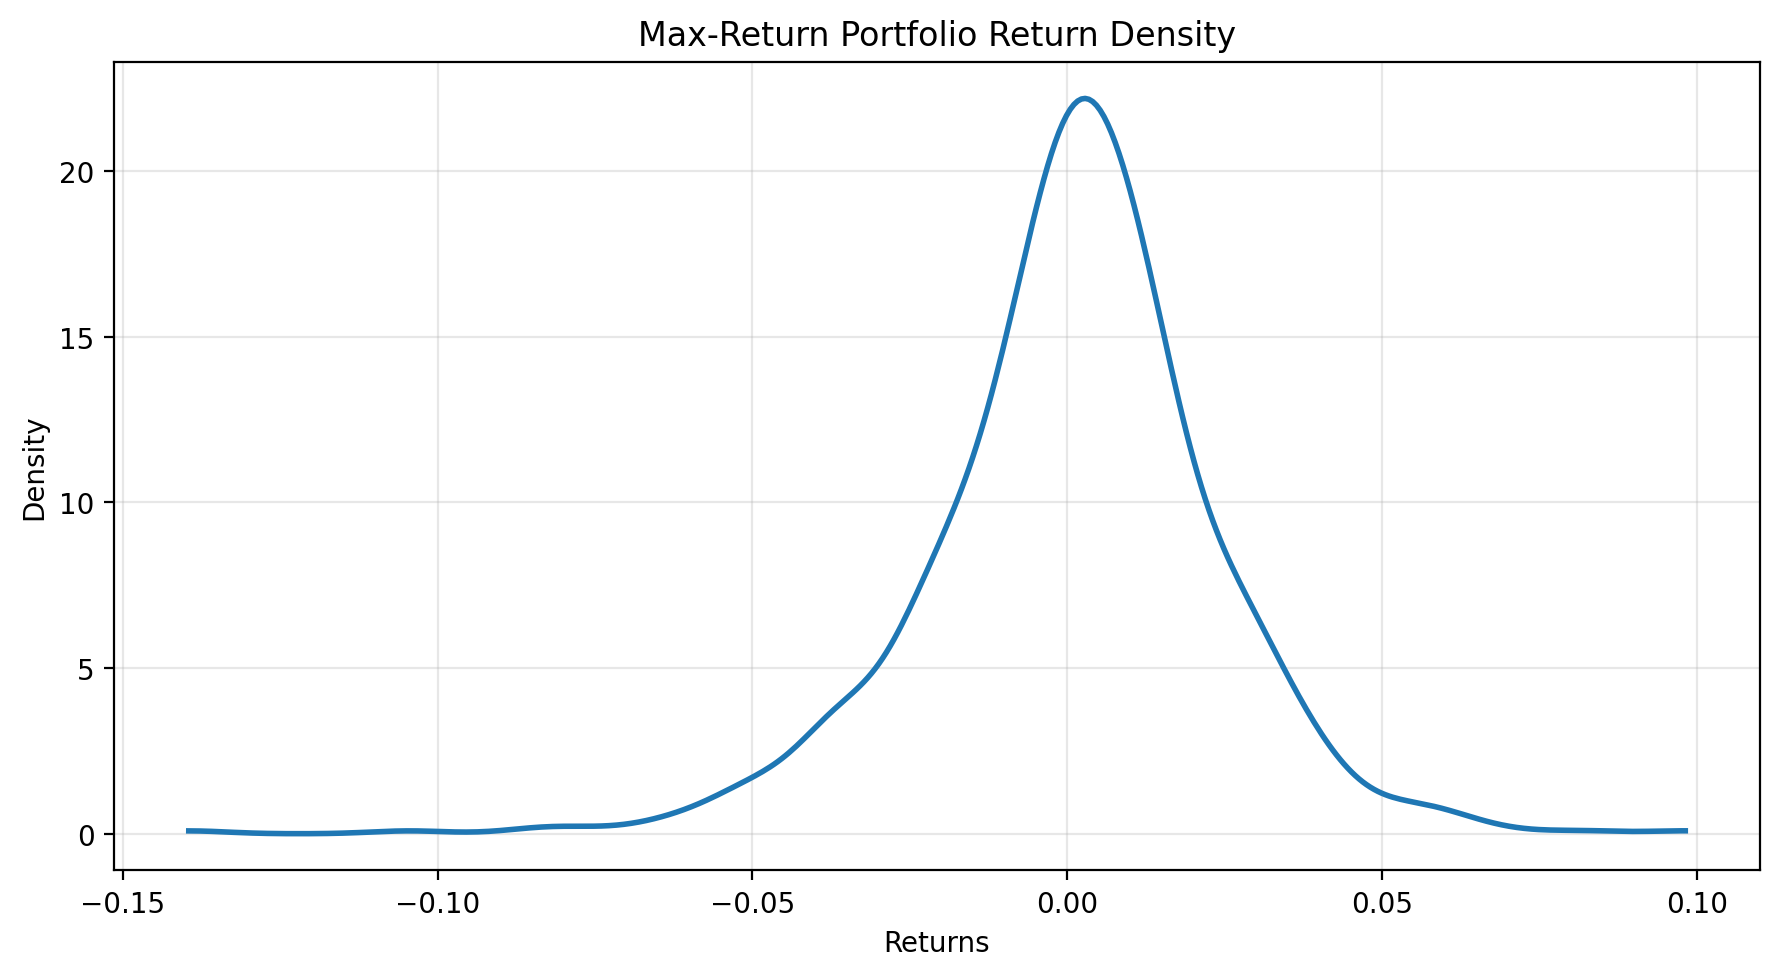
\includegraphics[width=0.8\textwidth]{outputs/figures/32_max_return_density.png}
\caption{Maximum-return portfolio return density}
\label{fig:maxret_density}
\end{figure}

\begin{figure}[H]
\centering
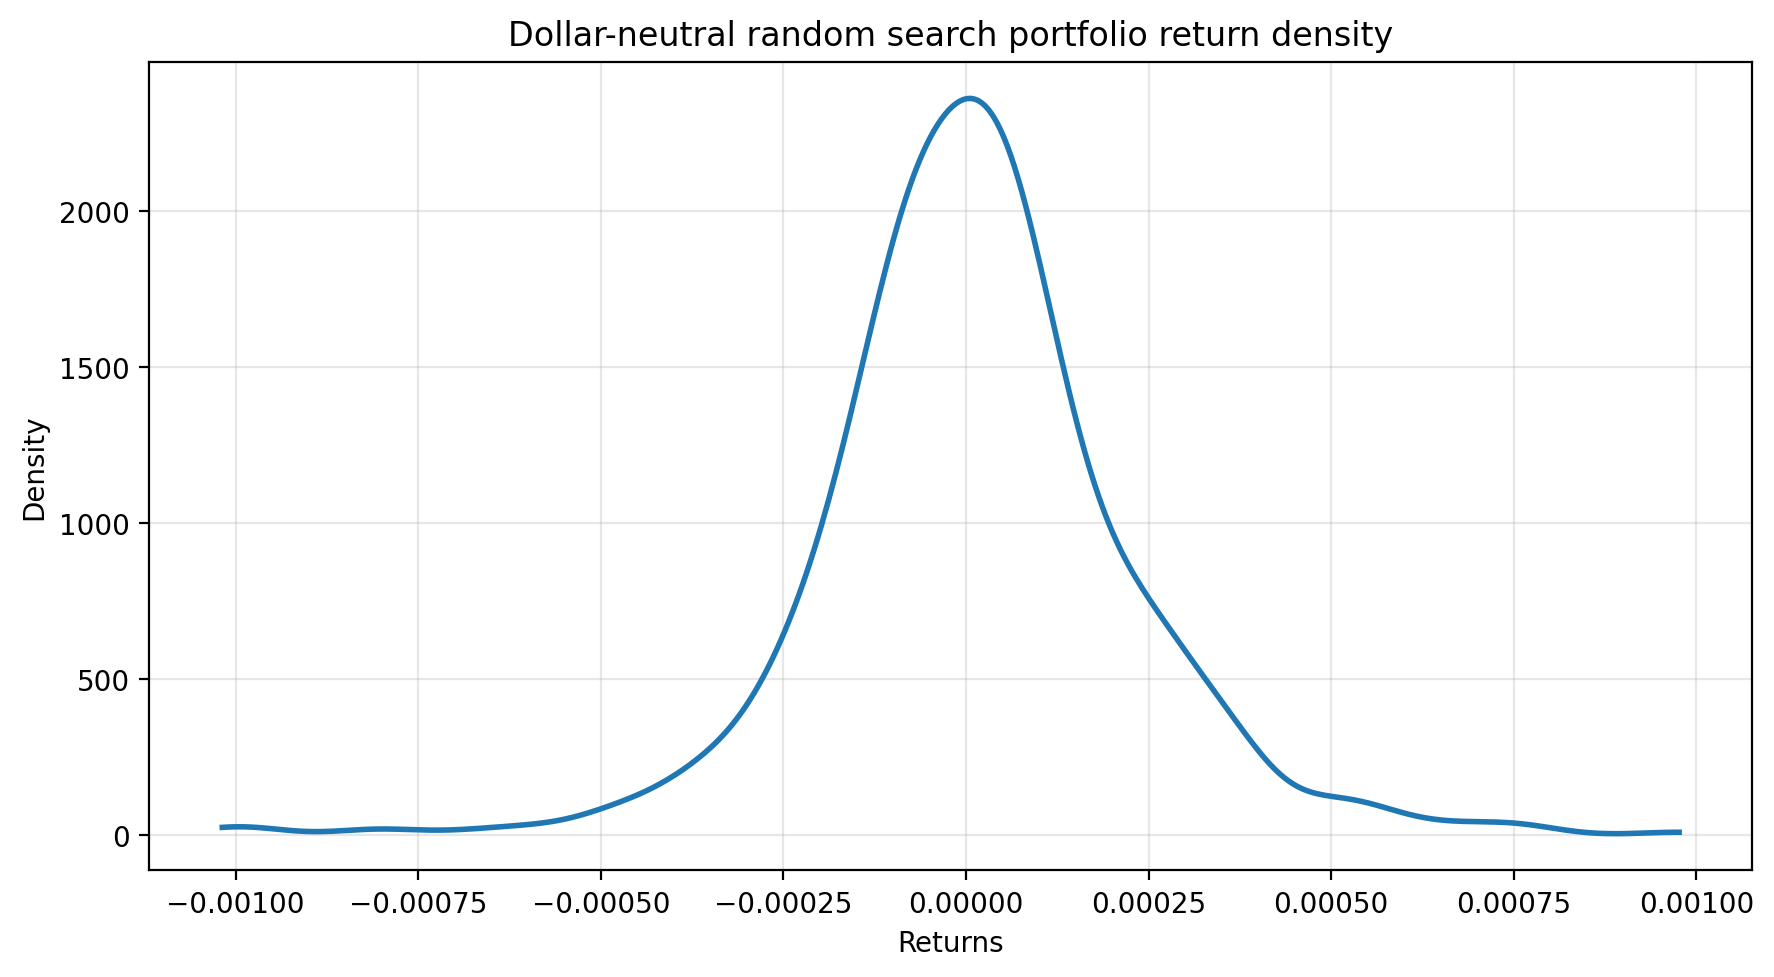
\includegraphics[width=0.8\textwidth]{outputs/figures/33_dollar_neutral_random_search_density.png}
\caption{Dollar-neutral portfolio return density}
\label{fig:dn_density}
\end{figure}

\begin{figure}[H]
\centering
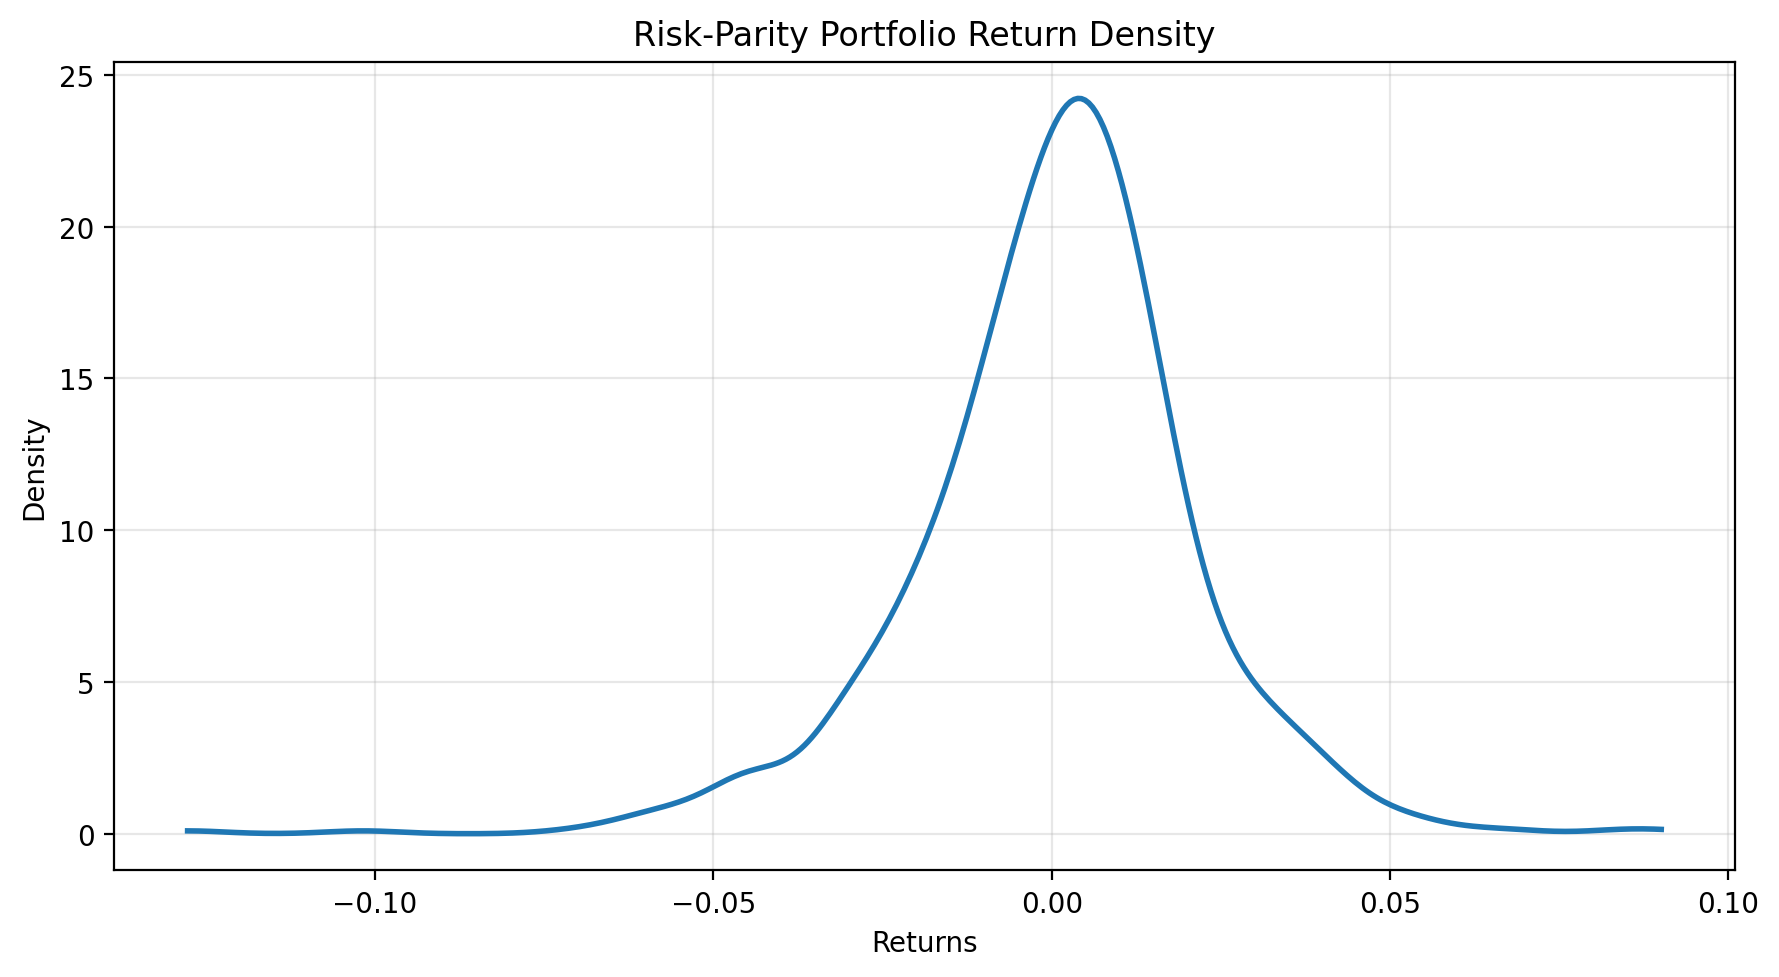
\includegraphics[width=0.8\textwidth]{outputs/figures/34_risk_parity_density.png}
\caption{Risk-parity portfolio return density}
\label{fig:rp_density}
\end{figure}

Figures \ref{fig:minvar_density}--\ref{fig:rp_density} show that the diversified long-only portfolios have broadly similar shapes, while the dollar-neutral density is much tighter around zero.

\begin{figure}[H]
\centering
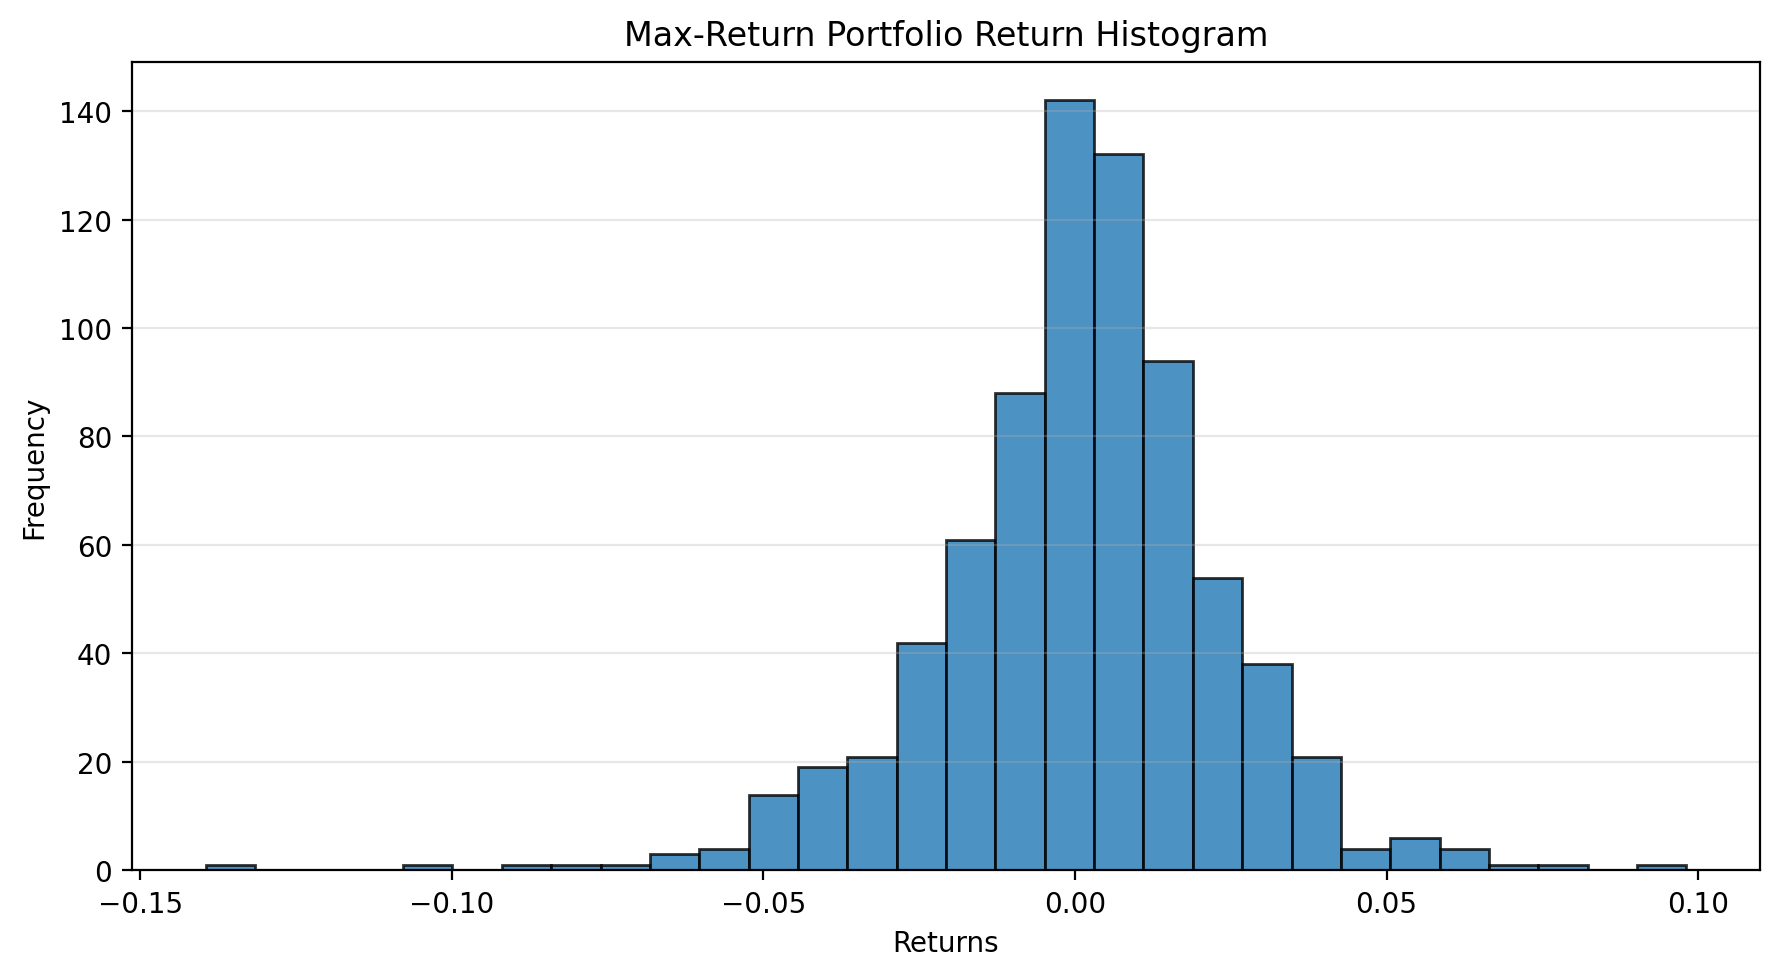
\includegraphics[width=0.8\textwidth]{outputs/figures/22_max_return_histogram.png}
\caption{Maximum-return portfolio return histogram}
\label{fig:maxret_hist}
\end{figure}

\begin{figure}[H]
\centering
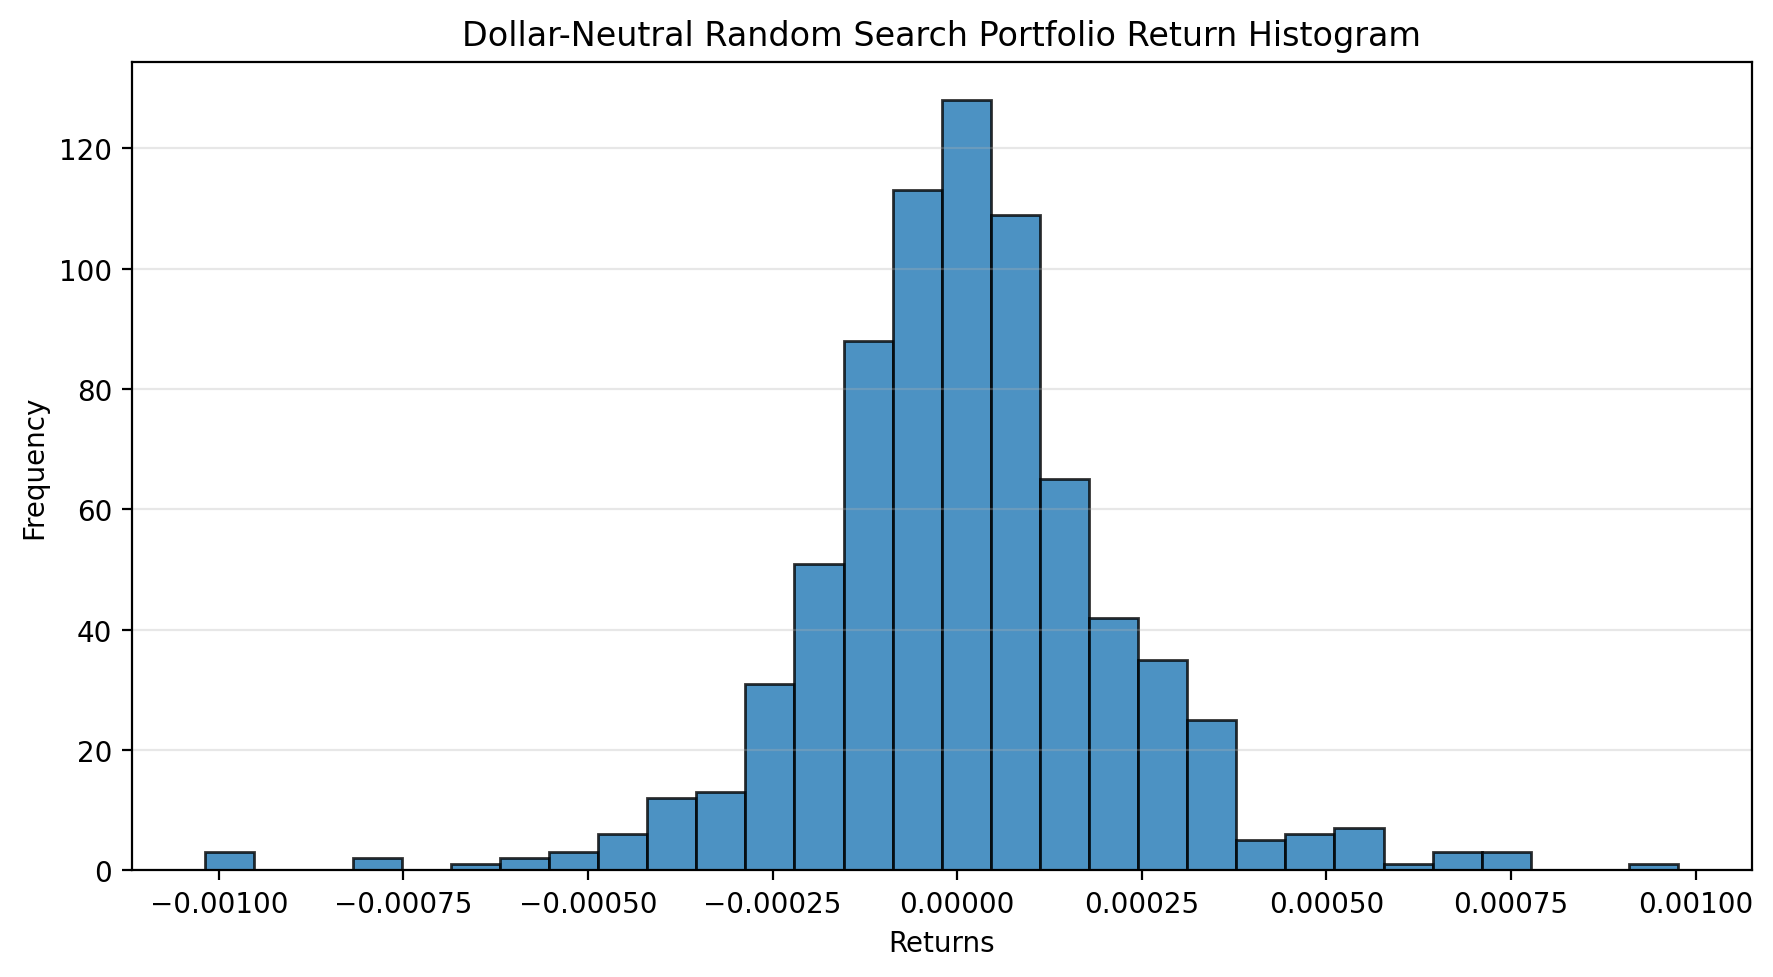
\includegraphics[width=0.8\textwidth]{outputs/figures/23_dollar_neutral_random_search_histogram.png}
\caption{Dollar-neutral random search portfolio return histogram}
\label{fig:dn_hist}
\end{figure}

\begin{figure}[H]
\centering
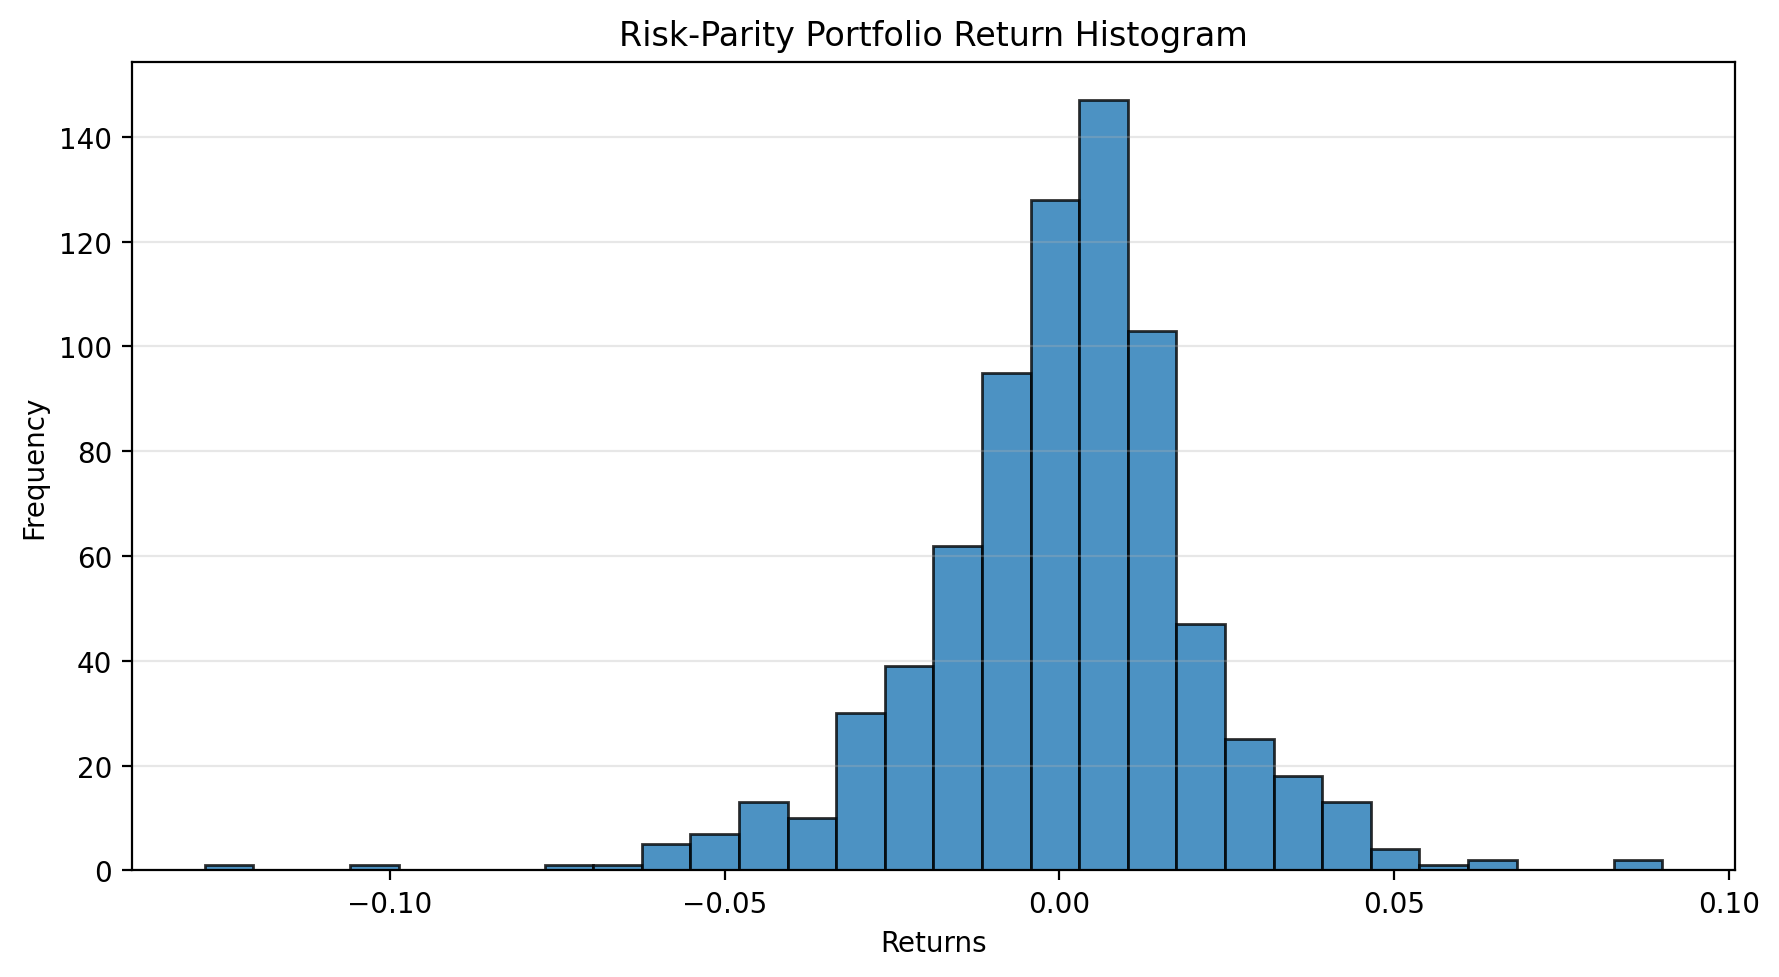
\includegraphics[width=0.8\textwidth]{outputs/figures/24_risk_parity_histogram.png}
\caption{Risk-parity portfolio return histogram}
\label{fig:rp_hist}
\end{figure}

\begin{figure}[H]
\centering
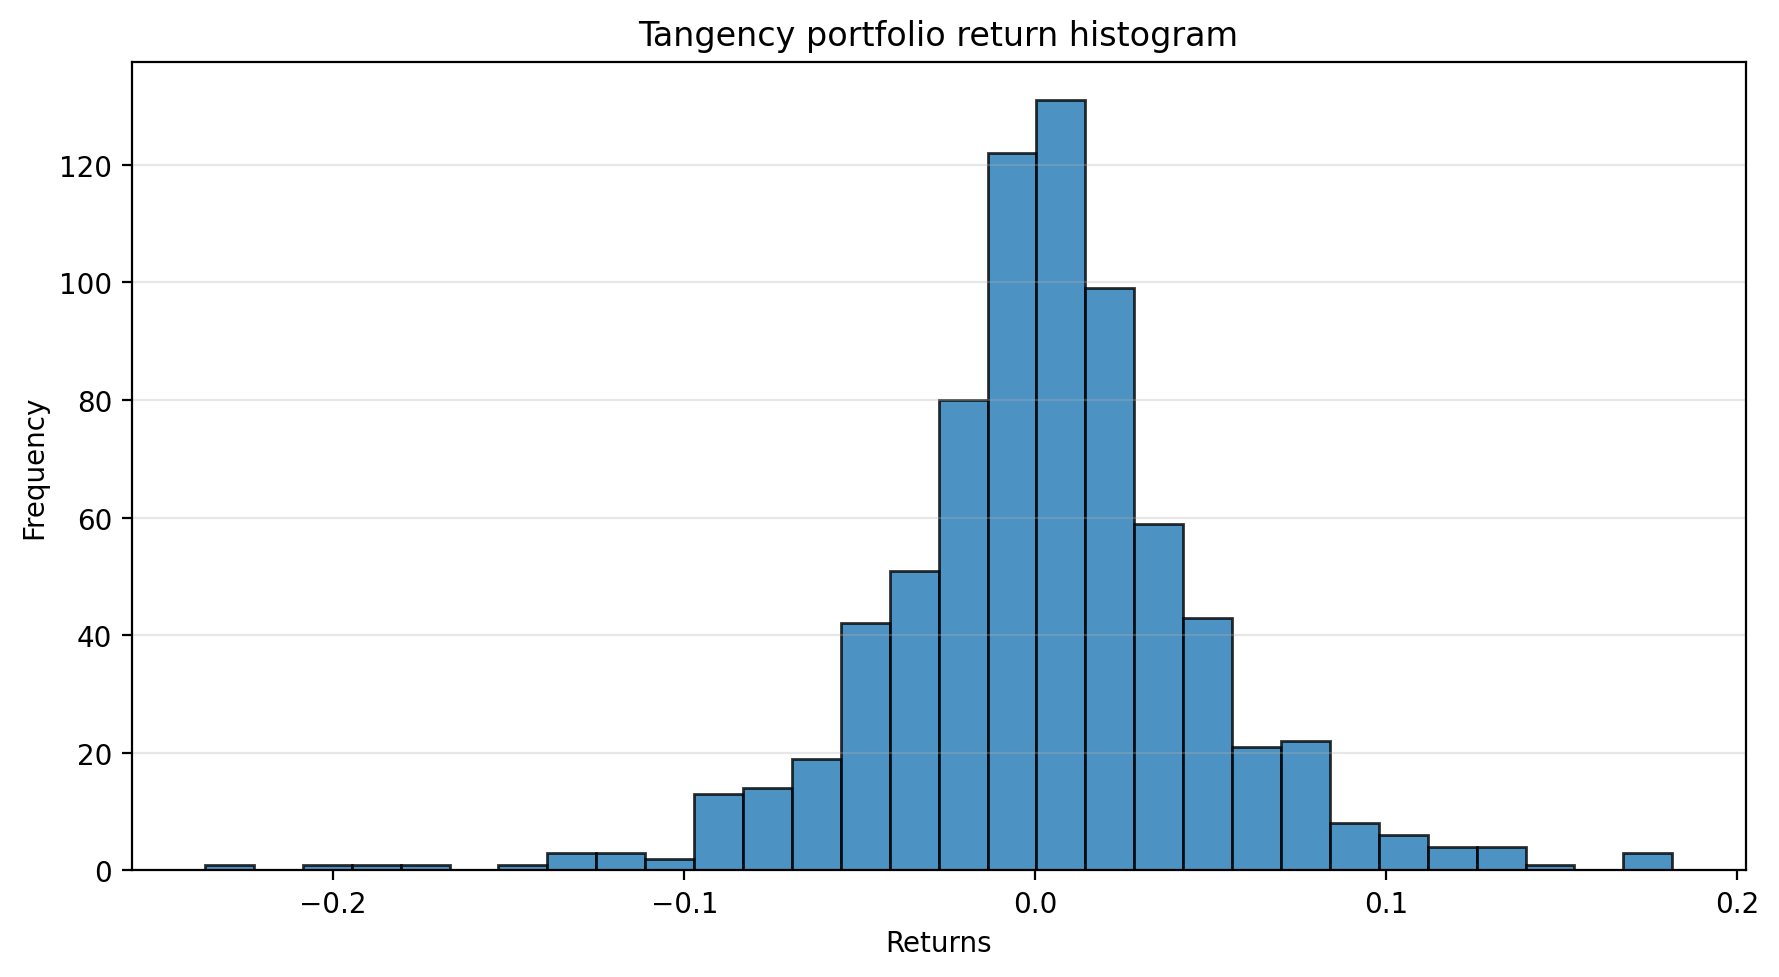
\includegraphics[width=0.8\textwidth]{outputs/figures/25_tangency_histogram.png}
\caption{Tangency portfolio return histogram}
\label{fig:tangency_hist}
\end{figure}

Figures \ref{fig:maxret_hist}--\ref{fig:tangency_hist} confirm that the dollar-neutral strategy is the most concentrated around zero, while the tangency portfolio is the widest and most dispersed. This aligns with the numerical results in Table \ref{tab:portfolio_summary}, where the dollar-neutral standard deviation is nearly zero and the tangency standard deviation is the largest.

\section{Exact Tangency Point and Utility-Based Choice}

Combining Figure \ref{fig:frontier} with Figure \ref{fig:indifference} yields the full economic interpretation of portfolio selection. The efficient frontier gives the feasible set of optimal risky portfolios, while the indifference curves determine which point on that frontier is preferred by a given investor.

For an investor with risk aversion coefficient $A$, the optimal risky allocation satisfies the tangency condition
\begin{equation}
\frac{d\mu_p}{d\sigma_p} = A \sigma_p.
\end{equation}
Thus:
\begin{itemize}
\item highly risk-averse investors choose points closer to the minimum-variance region;
\item less risk-averse investors choose points further up the frontier;
\item the portfolio with the highest Sharpe ratio provides the strongest reward-to-risk slope from the risk-free rate.
\end{itemize}

In the present sample, the tangency portfolio is also the highest-return optimized portfolio. This occurs because Tesla’s sample mean return is large enough relative to its volatility to dominate the Sharpe-ratio objective under the imposed constraints.

\section{CAPM Interpretation}

The Capital Asset Pricing Model (CAPM) links expected returns to exposure to the market portfolio:
\begin{equation}
E[R_i] = r_f + \beta_i \big(E[R_M] - r_f\big),
\end{equation}
where
\begin{equation}
\beta_i = \frac{\operatorname{Cov}(R_i, R_M)}{\operatorname{Var}(R_M)}.
\end{equation}

Within the mean-variance framework, the tangency portfolio plays the role of the market portfolio. When investors combine the risk-free asset with the tangency portfolio, the efficient frontier in risky-asset space gives rise to the Capital Market Line (CML). In that interpretation:
\begin{itemize}
\item the tangency portfolio is the unique risky portfolio held by all investors;
\item investors differ only in how much they lever or de-lever that portfolio;
\item the slope of the CML equals the Sharpe ratio of the tangency portfolio.
\end{itemize}

Although the present analysis is purely sample-based and not a formal CAPM test, it illustrates the core economic connection between mean-variance optimization and equilibrium asset pricing.

\section{Conclusion}

This study demonstrates how portfolio theory can be implemented in a modular Python workflow and interpreted through both statistical and economic lenses. The main findings are:
\begin{itemize}
\item Tesla has the largest average return and the largest volatility.
\item Diversified portfolios such as minimum-variance and risk parity produce materially lower risk than the tangency solution.
\item The dollar-neutral strategy behaves as designed, remaining tightly centered around zero with minimal dispersion.
\item The tangency portfolio maximizes the return-to-risk trade-off in the sample and becomes fully concentrated in Tesla.
\item Indifference curves provide the missing investor-preference layer needed to translate the efficient frontier into an actual portfolio choice.
\end{itemize}

Overall, the report shows that markets determine the efficient set of risky opportunities, while investor preferences determine which point on that set is ultimately chosen.

\end{document}